\chapter{Resultados} \label{cap:resultados}
    Este capítulo reúne os resultados das 2 fases experimentais deste trabalho e seleciona por fim o melhor resultado entre as fases.
    
    A primeira fase experimental na etapa de pré-processamento realiza antes do desenvolvimento dos modelos, o procedimento de análise exploratória dos dados fundamentado no trabalho de \cite{Junior2007}.
    
    O parâmetro ``ENTR\_ALMOCO'' da tabela \ref{table:dataset_final} é o atributo alvo da predição, pois se trata do número de entradas no ponto de acesso do restaurante, portanto esse parâmetro é frequentemente utilizado nos gráficos comparativos em formato de linha, sendo geralmente comparado com algum outro parâmetro de entrada nos modelos, denominado de ``Feature'' neste trabalho, nomenclatura utilizada por reconhecidas referências na área de Data Science, conforme o artigo de \cite{TWDSFeatures}.
    
    Nesta primeira fase também são desenvolvidos 2 modelos de redes MLP para suporte na análise exploratória do problema da predição do restaurante e é verificado se esses modelos tem capacidade de aprendizado sobre o problema.
    
    Depois de verificada a capacidade de aprendizado do problema foram desenvolvidos 3 modelos endógenos, sendo uma rede MLP e duas redes GRU. Os resultados de predição foram comparados visando a seleção do melhor modelo endógeno.
    
    Após a seleção do melhor modelo, foram desenvolvidos três modelos mistos. Ao contrário dos anteriores, estes modelos recebem como entrada tanto features endógenas quanto exógenas. Da mesma forma, o melhor modelo com ambas as features também é selecionado.
    
    %Ao fim da fase é comparado o melhor modelo entre o melhor endógeno e o melhor modelo misto.
    
    Na segunda fase, é alterado o domínio temporal experimental para a divisão dos conjuntos e repetidos os passos da primeira fase a partir do desenvolvimento dos modelos endógenos.
    
    Após selecionado o melhor modelo da segunda fase, foram comparados os melhores modelos das duas fase. Para uma comparação justa, visto que o melhor modelo da 1a fase tem domínio de teste restrito ao primeiro semestre de 2019, o modelo obtido na segunda fase é novamente testado apenas no domínio do primeiro semestre obtendo-se novas métricas de teste.
    
    
    Ao final das duas fases experimentais, o modelo com melhor predição dos dados é apresentado como um possível preditor para a demanda do RU.
    %Por fim é selecionado o melhor modelo de todas as fases experimentais para a conclusão do trabalho.
     
	\section{Fase Experimental I}
	     \begin{figure}[htb]
        	\center{
        		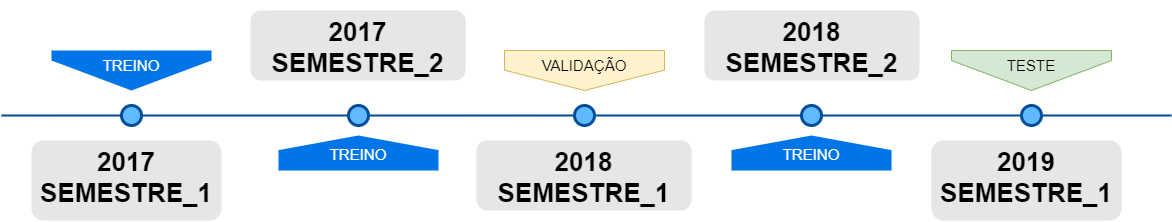
\includegraphics[width=1.0\textwidth]{./Figuras/resultados/case1_timeline.png}
        	
        	\caption{Domínio temporal da 1a fase} \label{fig:case1_timeline} }
        \end{figure}
	    O domínio experimental desta fase segue de acordo com a figura \ref{fig:case1_timeline}.
	    Nesta fase temos 1 modelo selecionado na comparação de resultados entre 3 modelos endógenos e 3 modelos exógenos desenvolvidos, treinados e testados.
	    A hipótese sobre este modelo segue sobre o seu conjunto de validação que contempla apenas o primeiro semestre de 2018, portanto é o indicado para semestres com sazonalidade, grade horária de disciplinas e comportamento de consumo semelhante ao 1o semestre de 2018.
	    
	    \subsection{Pré-Processamento}
	        Nesta subseção é realizada, no conjunto de treino, a análise exploratória das features e do comportamento de consumo, e também executada a técnica atual de previsão do restaurante no conjunto de teste, composta pela produção de refeições, para cada dia, com margem de 30\% acima do consumo do mesmo dia da semana anterior.
	       % \newpage
    	    \subsubsection{Divisão dos conjuntos}
    	        
    	        \paragraph{Dificuldades encontradas e resolvidas}
    	            A primeira dificuldade encontrada foi um comportamento anômalo do gráfico de previsão e valores reais. O conjunto de dados foi lido trocando datas (dia por mês e mês por dia). A indexação por data na divisão de conjuntos produzia gráficos fora do formato esperado, de acordo com a figura \ref{fig:pandas_wrong_indexing}.
    	            
    	            \begin{figure}[htb]
                    	\center{
                    		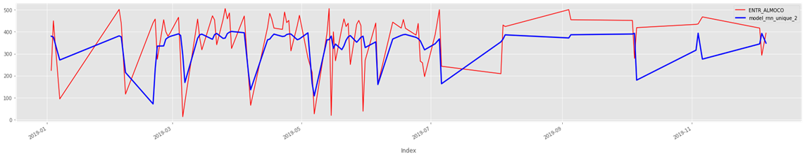
\includegraphics[width=1.0\textwidth]{./Figuras/resultados/pandas_wrong_indexing.png}
                    	
                    	\caption{Resultado do modelo RNN\_ENDO\_2 obtido sobre o conjunto de dados aleatoriamente ordenado sobre o tempo} \label{fig:pandas_wrong_indexing} }
                    \end{figure}

                    Corrigindo a importação dos registros para o padrão brasileiro na ferramenta pandas os resultados foram melhores e condizentes com o comportamento real de consumo, além disso nota-se que a primeira fase filtra dados obtidos apenas para o 1o semestre de 2019 e no caso da indexação incorreta na figura \ref{fig:pandas_wrong_indexing} a ordenação ultrapassou o mês de julho, este foi o comportamento que indicou a investigação no código de importação.
                    
                    \begin{figure}[htb]
                    	\center{
                    		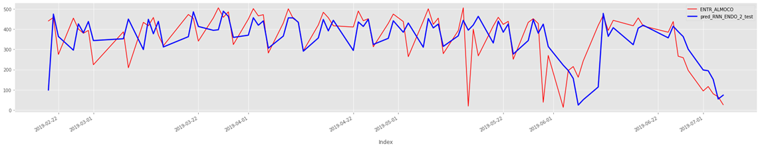
\includegraphics[width=1.0\textwidth]{./Figuras/resultados/pandas_correct_indexing.png}
                    	
                    	\caption{Resultado do modelo RNN\_ENDO\_2 obtido sobre o conjunto de dados com ordenação corrigida \label{fig:pandas_correct_indexing} }}
                    \end{figure}
                    
                    A figura \ref{fig:pandas_correct_indexing} demonstra os resultados obtidos após a correção da leitura dos dados, onde todos os modelos obtiveram resultados melhores. 
                    Isto também demonstra que ordenações aleatórias na divisão dos conjuntos de treino, teste e validação, não seriam indicadas para a execução deste trabalho.
                    %%%%
                    %TODO-T: CITAR FIGURAS
                    % \newpage
                    Nas figuras \ref{fig:case1_train} , \ref{fig:case1_val} e \ref{fig:case1_test}   são exibidos os valores reais de consumo nos conjuntos de treino (2017-1,2017-2,2018-2), validação (2018-1) e teste (2019-1).
                    {  \begin{center}
                    %TREINO
                    \begin{minipage}[c]{0.45\textwidth}
                        \begin{figure}[H]
                        	\center{                    		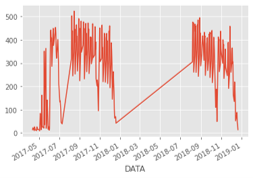
\includegraphics[width=\textwidth]{./Figuras/resultados/case1_train.png}
                        	\caption{1a fase, Conjunto verdade de treino} 
                        	\subcaption{Dados do 1o e 2o semestre de 2017 \newline e 2o semestre de 2018.} \label{fig:case1_train} }
                        \end{figure}
                        %VALIDACAO }
                        \end{minipage} \hfill %
                          \begin{minipage}[c]{0.45\textwidth}
                        \begin{figure}[H]
                        	\center{                    		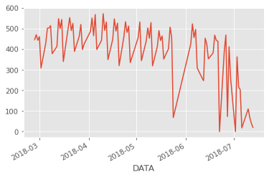
\includegraphics[width=\textwidth]{./Figuras/resultados/case1_val.png}
                        	\caption{1a fase, Conjunto verdade de validação}
                        	\subcaption{Dados  do 1o semestre de 2018.	} \label{fig:case1_val} }
                        \end{figure}%
                    %TESTE
                    \end{minipage}
                    \begin{minipage}[c]{1.0\textwidth}
                        \begin{figure}[H]
                        	\center{                    	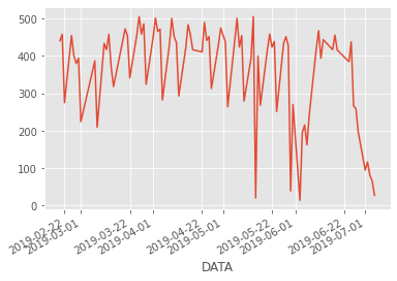
\includegraphics[width=0.9\textwidth]{./Figuras/resultados/case1_test.png}
                        	 \caption{1a fase, Conjunto verdade de teste} \subcaption{Dados do 1o semestre de 2019.} \label{fig:case1_test} }
                        \end{figure}
                    \end{minipage} \end{center} }
            % \newpage
            
    	    \subsubsection{Análise das variáveis endógenas}
    	       
    	        \paragraph*{Consumo em relação às vendas de 1 dia anterior}
        	       {
        	       \begin{center} 
            	        \begin{minipage}[c]{1.0\textwidth}
            	            \begin{figure}[H]
                            	\center{                    		        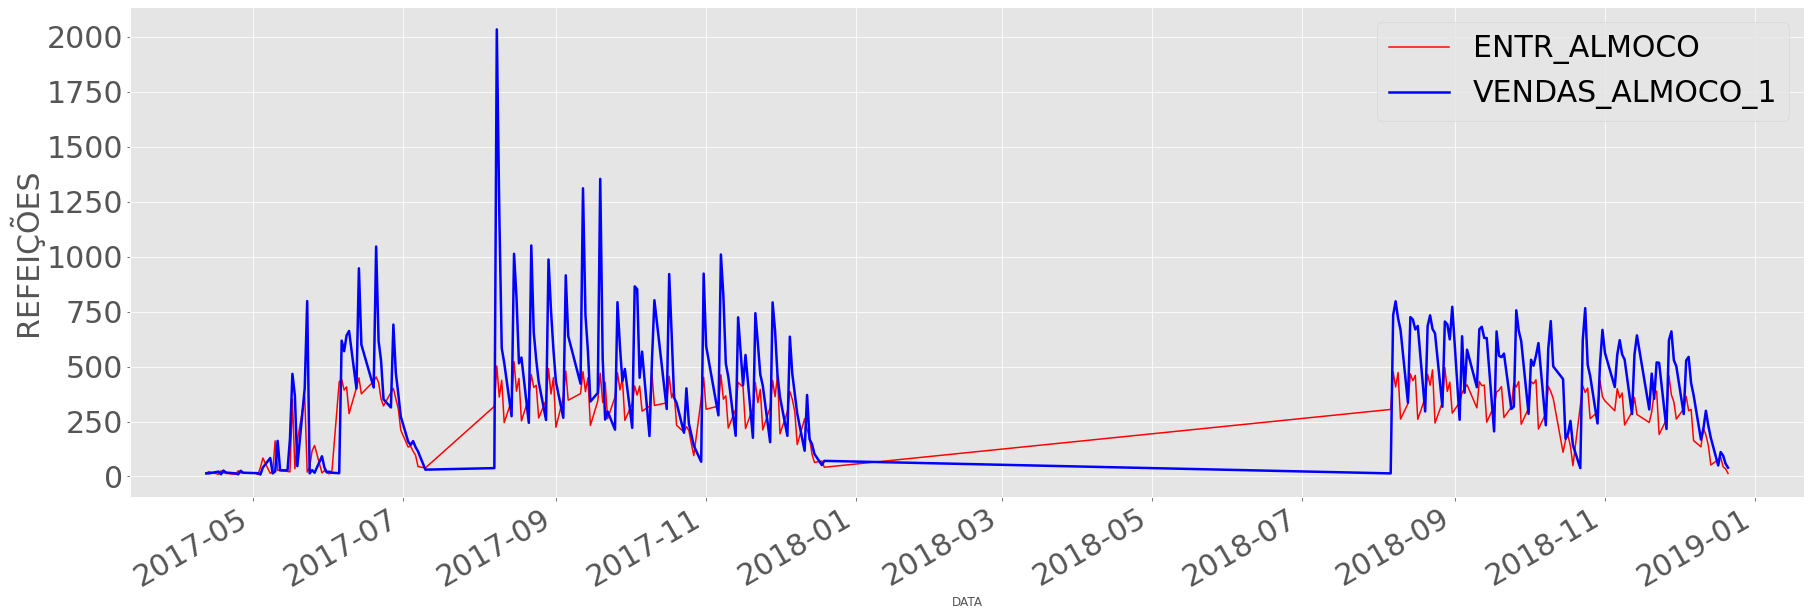
\includegraphics[width=1.0\textwidth]{./Figuras/resultados/case1_consumo_vendas_almoco.png}
                            	\caption{Correlação entre consumo e vendas de almoço.} \label{fig:case1_consumo_vendas_almoco} 
                            	}
                            \end{figure}
                        \end{minipage} \hfill %
                        \begin{minipage}[c]{0.3\textwidth}
                            \begin{figure}[H]
                            	\center{                    		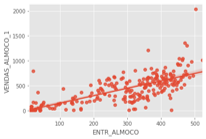
\includegraphics[width=1.0\textwidth]{./Figuras/resultados/case1_scatter_consumo_vendas_almoco.png}
                            	\caption{Gráfico Scatter entre consumo e vendas de almoço.} \label{fig:case1_scatter_consumo_vendas_almoco} }
                            \end{figure}
                        \end{minipage} 
                    \end{center}
                    }
                        
                   \begin{table}[!ht]
                   \centering
                   \caption{Comparação de consumo com um dia anterior}
                     \rowcolors{2}{gray!25}{white}
                     \begin{tabular}{|c|c|}\hline
                        \multicolumn{2}{c}{CONSUMO EM RELAÇÃO ÀS VENDAS DE 1 DIA ANTERIOR}\\ \hline
                            CORRELAÇÃO (r) &  0.7255528038157009\\
                            P-value &5.399561176138223e-41\\
                            RMSE & 260.5399426736619\\
                            TOTAL DE REFEIÇÕES PROJETADAS & 104694\\ 
                            TOTAL DE REFEIÇÕES CONSUMIDAS & 69544\\
                            TOTAL DE REFEIÇÕES SUB PROJETADAS & -4703\\
                            TOTAL DE REFEIÇÕES SUPER PROJETADAS & 39853\\
                            ERRO ABSOLUTO MEDIANO & 139.0\\
                            ERRO ABSOLUTO PERCENTUAL MEDIO & 90.18\\\hline
                    \end{tabular} \label{table:case1_vendas1} \end{table}

        	       % \newpage
        	        É possível notar na figura \ref{fig:case1_consumo_vendas_almoco} que as vendas de ticket de almoço apresentaram comportamento diferente no ano de 2017 em comparação aos anos seguintes devido à uma limitação imposta pelo restaurante, a partir de 2018, que os alunos comprassem apenas 2 tickets por dia. Possivelmente esta limitação foi dada para aproximar o comportamento de consumo de 1 até 2 dias seguintes à vendas de tickets no dia vigente, esta limitação pode ser interpretada como método de auxílio à gestão para a produção de refeições e para o tratamento de desperdício.
            	        
        	        Mesmo com o outlier de 2000 vendas em um dia, e com a nova limitação de compras de tickets a partir de 2018, o consumo está fortemente relacionado com as vendas de tickets de 1 dia anterior e que os alunos se adaptaram à utilização em curto prazo dos tickets, conforme o valor de correlação aproximado em 72\% que pode ser conferido na tabela \ref{table:case1_vendas1}.
        	        
        	        Há outros fatores não previstos envolvidos, como falha de registros no sistema, bem como o outlier de 2000 vendas pode ser interpretado com a migração de sistema que ocorreu em 2017 da unidade talim do ICT Unifesp para o banco de dados do Hospital São Paulo, possivelmente foram importadas vendas do sistema antigo sem a diferenciação de datas.

                % \newpage
                \paragraph*{Normalização e escala de features}
                    O processo de normalização e escala é demonstrado nesta seção com a feature de vendas de tickets de 1 dia anterior, da seção anterior, pois entre todas as features esta é a que produziu outliers com maior destaque.
                    A normalização dos dados é feita com o teto de 3x o desvio padrão médio, logo o pico de 2000 vendas foi normalizado para o valor arredondado de 1356 refeições e mesmo com a normalização, o comportamento linear desta feature, conforme figura \ref{fig:feature_sem_outliers}, se manteve.   
                    E após a normalização foi realizada a aplicação da escala de 0 a 1 na feature e conforme é observado na figura  \ref{fig:feature_sem_outliers_escalada}, o comportamento linear da feature também se manteve.

                    {
                        \begin{center}
                            \begin{minipage}[b]{1.0\textwidth}
                            \begin{figure}[H]
                            	\center{
                                	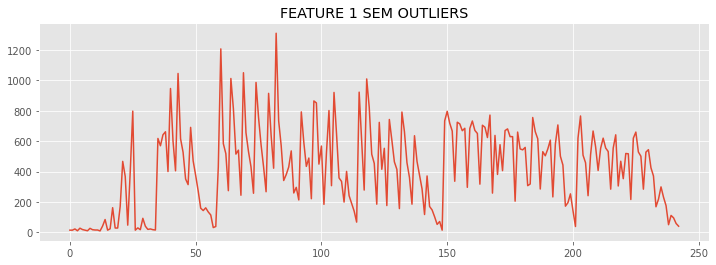
\includegraphics[width=1.0\textwidth]{./Figuras/resultados/feature_sem_outliers.png}
                                	\caption{Vendas de tickets normalizados com teto de 3x o desvio padrão.}
                                	\label{fig:feature_sem_outliers}
                            	}
                            \end{figure}
                            \end{minipage} \hfill %
                            
                            \begin{minipage}[b]{1.0\textwidth}
                            \begin{figure}[H]
                            	\center
                            	{                    		
                                	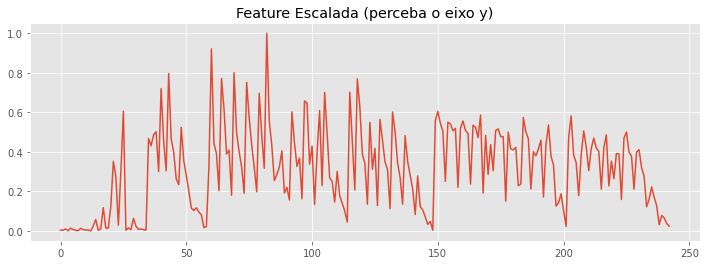
\includegraphics[width=1.0\textwidth]{./Figuras/resultados/feature_sem_outliers_escalada.png}
                                	\caption{Vendas de tickets escalada entre 0 a 1.} \label{fig:feature_sem_outliers_escalada} 
                            	}
                            \end{figure}
                            \end{minipage}
                        \end{center}
                    }
                    Este processo de normalização e escala foi realizado para todas as features endógenas e para as features climáticas.
        	   % \newpage
        	   
        	    \paragraph{Análise da técnica do restaurante}
        	       
        	        {
            	        \begin{center} 
                	        \begin{minipage}[c]{1.0\textwidth}
                	         \begin{figure}[H]
                            	\center{                		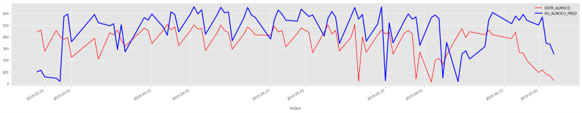
\includegraphics[width=1.0\textwidth]{./Figuras/resultados/case1_ru_pred.png}
                            	\caption{Correlação entre consumo e produção com 30\% acima do consumo da semana anterior.	} \label{fig:case1_ru_pred} }
                            \end{figure}
                            \end{minipage} \hfill %
                            
                            \begin{minipage}[c]{1.0\textwidth}
                                \begin{figure}[H]
                                	\center{                		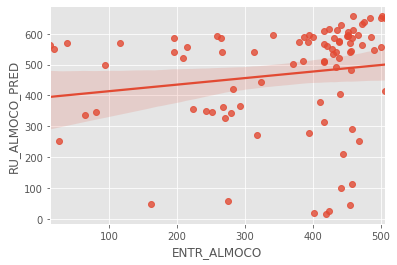
\includegraphics[width=0.5\textwidth]{./Figuras/resultados/case1_ru_pred_scatter.png}
                                	\caption{Gráfico Scatter entre consumo e produção com margem de 30\%. acima do consumo da semana anterior} \label{fig:case1_ru_pred_scatter} }
                                \end{figure}
                            \end{minipage} 
                        \end{center}
                    }
                     \begin{table}[!ht]
                       \centering
                         \rowcolors{2}{gray!25}{white}
                         \begin{tabular}{|c|c|}\hline
                            \multicolumn{2}{c}{Consumo vigente em relação ao 5o dia anterior}\\ \hline
                                CORRELAÇÃO (r): & 0.1593\\
                                Pi (p) : & 0.1380\\
                                RMSE = & 224.4733\\
                                TOTAL DE REFEIÇÕES PROJETADAS = & 41351\\ 
                                TOTAL DE REFEIÇÕES CONSUMIDAS = & 31962\\
                                TOTAL DE REFEIÇÕES SUB PROJETADAS = & -3650\\
                                TOTAL DE REFEIÇÕES SUPER PROJETADAS = & 13039\\
                                ERRO ABSOLUTO MEDIANO = & 152.0\\
                                ERRO ABSOLUTO PERCENTUAL MÉDIO = & 167.2659\% \\\hline
                        \end{tabular}
                        \caption{Estimações do restaurante para o 1o Semestre de 2019}
                        \label{table:case1_rupred}
                    \end{table}
                    
        	        A análise da técnica de estimação de consumo, do restaurante, foi feita com o cálculo de 30\% de produção acima do consumo do 5o dia anterior.
        	        É possível notar que o modelo do R.U é feito para tolerar descartes devido à multa contratual para falta de refeições e o que a produção de 30\% de refeições acima do consumo da semana anterior, conforme a figura  \ref{fig:case1_ru_pred} produz um comportamento linear distante do comportamento real de consumo, apesar de seguir as tendễncias de quedas e aumento de consumo, na figura \ref{fig:case1_ru_pred_scatter} do gráfico scatter gerada pela biblioteca seaborn também demonstra que a regressão linear (representada pela linha vermelha no gráfico) tem o eixo totalmente descentralizado com a função identidade entre o consumo e a predição ideal (representada pela diagonal formada entre a origem do gráfico e o vértice superior direito), gerando também um erro muito maior do que 30\% no somatório total de refeições descartadas no semestre, devido ao comportamento oscilatório do consumo, conforme a tabela \ref{table:case1_rupred}.
                \paragraph{Consumo atual em relação ao consumo do jantar de 1 dia anterior.}
                
                    Apesar de que os alunos que consomem refeições no almoço geralmente são de período e  de grade horária diferente dos alunos que consomem o jantar no período da noite, nota-se uma relação evidente entre os 2 consumos, evidenciada pelo comportamento linear na figura \ref{fig:case1_consumo_jantar} com correlação (r) = 0.7655, e pela regressão linear entre esses 2 consumos na figura  \ref{fig:case1_consumo_jantar_scatter}.\newline
                    
                    {\begin{center} 
                    \begin{minipage}[c]{1.0\textwidth}
                    \begin{figure}[H]
                    	\center{
                    	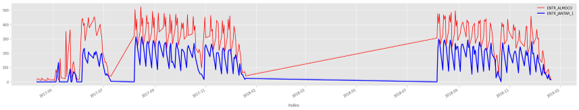
\includegraphics[width=1.0\textwidth]{./Figuras/resultados/case1_consumo_jantar.png}
                    	\caption{Correlação de consumo de almoço e jantar de 1 dia anterior.} 
                    	\label{fig:case1_consumo_jantar} }
                    \end{figure} 
                    \end{minipage}\hfill %
                    
                    \begin{minipage}[c]{0.3\textwidth}
                    \begin{figure}[H]
                    	\center{                    		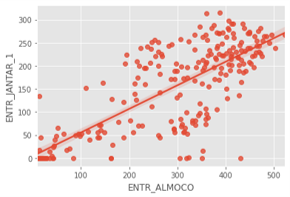
\includegraphics[width=1.0\textwidth]{./Figuras/resultados/case1_consumo_jantar_scatter.png}
                    	\caption{Gráfico Scatter entre consumo e jantar de 1 dia anterior.} 
                    	\label{fig:case1_consumo_jantar_scatter} }
                    \end{figure}
                    \end{minipage} \end{center} }
            
    	    \subsubsection{Análise da sazonalidade semanal}
    	        Os gráficos a seguir da figura  \ref{fig:case1_violinplot_segunda}, representando a segunda-feira,  até a figura \ref{fig:case1_violinplot_sexta} , representando a sexta-feira,  são gerados para as features categóricas binárias, com a funcionalidade violin-plot da biblioteca seaborn, própria para distribuição de variáveis categóricas-binárias em um dataset.
    	        O violino azul com o valor 1 representa a distribuição do consumo ao logo do dataset.
    	        O violino com valor zero pode ser ignorado e é um retorno padrão da ferramenta, representando a distribuição da ausência de consumo no dia da semana considerado.
    	        Nas sextas feiras, o consumo teve escala de distribuição menor para o primeiro semestre de 2019.
    	       %\newpage
    	       \begin{center}    
    	        \begin{minipage}[c]{0.45\textwidth}
    	         \begin{figure}[H]
                	\center{                		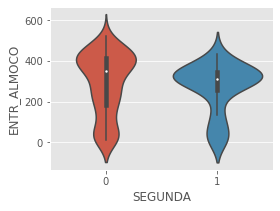
\includegraphics[width=\textwidth]{./Figuras/resultados/case1_segunda.png}
                	\caption{Gráfico violino da distribuição do consumo na segunda feira.} \label{fig:case1_violinplot_segunda} }
                \end{figure}\end{minipage} \hfill %
                      \begin{minipage}[c]{0.45\textwidth}
                \begin{figure}[H]
                	\center{                		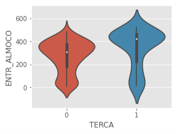
\includegraphics[width=\textwidth]{./Figuras/resultados/case1_terca.png}
                	\caption{Gráfico violino da distribuição do consumo na terça feira.} \label{fig:case1_violinplot_terca} }
                \end{figure} \end{minipage}
                 \begin{minipage}[c]{0.45\textwidth} 
                \begin{figure}[H]
                	\center{                		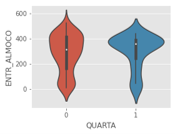
\includegraphics[width=\textwidth]{./Figuras/resultados/case1_quarta.png}
                	\caption{Gráfico violino da distribuição do consumo na quarta feira.	} \label{fig:case1_violinplot_quarta} }
                \end{figure}\end{minipage} \hfill %
                      \begin{minipage}[c]{0.45\textwidth}
                \begin{figure}[H]
                	\center{                		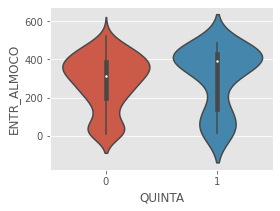
\includegraphics[width=\textwidth]{./Figuras/resultados/case1_quinta.png}
                	\caption{Gráfico violino da distribuição do consumo na quinta feira.} \label{fig:case1_violinplot_quinta} }
                \end{figure}\end{minipage} %
                        \begin{minipage}[c]{0.45\textwidth}
                \begin{figure}[H]
                	\center{                		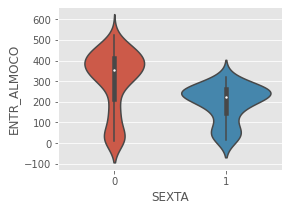
\includegraphics[width=\textwidth]{./Figuras/resultados/case1_sexta.png}
                	\caption{Gráfico violino da distribuição do consumo na sexta feira.} \label{fig:case1_violinplot_sexta} }
                \end{figure}
                \end{minipage} \end{center} 
            
            % \newpage
    	    \subsubsection{Análise das variáveis exógenas}
    	        \paragraph{Consumo atual em relação ao avanço do semestre}
    	            {
                    \begin{center} 
                    
                        \begin{minipage}[c]{1.0\textwidth}
                            \begin{figure}[H]
                            	\center{                    		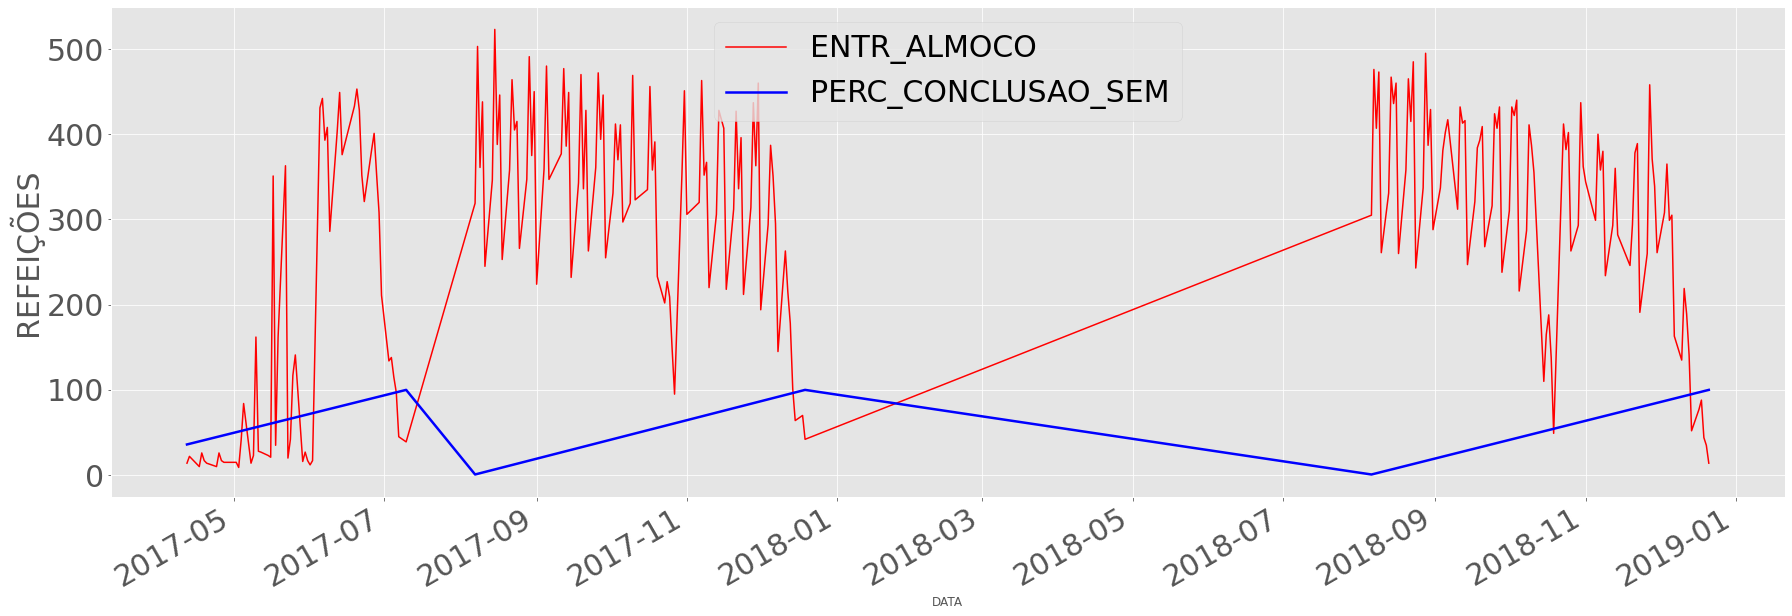
\includegraphics[width=\textwidth]{./Figuras/resultados/case1_perc_sem.png}
                            	\caption{Relação da distribuição do consumo com o avanço do semestre.}
                            	\subcaption{Correlação (r) = -0.3513, p-value = 1.8029942608003656e-08}
                            	\label{fig:case1_perc_sem}
                            	}
                            \end{figure}  
                        \end{minipage} \hfill %
                    
                        \begin{minipage}[c]{0.5\textwidth}
                            \begin{figure}[H]
                            	\center{                		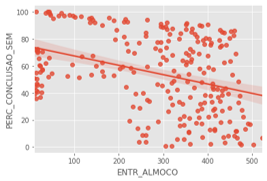
\includegraphics[width=\textwidth]{./Figuras/resultados/case1_perc_sem_scatter.png}
                            	\caption{Gráfico scatter da distribuição do consumo com o avanço do semestre.} \label{fig:case1_perc_sem_scatter}
                            	}
                            \end{figure}
                        \end{minipage} 
                    
                    \end{center} 
                    }
    	            Na correlação do consumo em relação ao avanço do semestre, para os últimos dias do semestre o consumo teve queda abrupta, a correlação dos conjuntos de dados das figuras \ref{fig:case1_perc_sem} e \ref{fig:case1_perc_sem_scatter} obtém valor negativo mas devido às oscilações de consumo, a correlação não se torna significativa.
    	      
    	   %   \newpage
              \paragraph{Consumo atual em relação ao avanço do mês}
                
                {
                \begin{center} 
                    \begin{minipage}[c]{0.45\textwidth}
                        \begin{figure}[H]
                        	\center{
                            	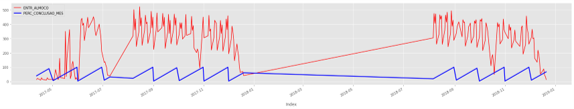
\includegraphics[width=\textwidth]{./Figuras/resultados/case1_perc_mes.png}
                            	\caption{Relação da distribuição do consumo com o avanço do mês.}
                            	\subcaption{Correlação (r) = 0.04867}
                            	\label{fig:case1_perc_mes} 
                        	}
                        \end{figure}
                    \end{minipage} \hfill %
                    
                    \begin{minipage}[c]{0.5\textwidth}
                    \begin{figure}[H]
                    	\center{                		
                        	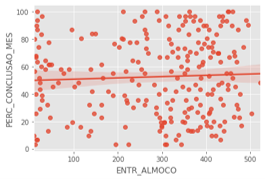
\includegraphics[width=\textwidth]{./Figuras/resultados/case1_perc_mes_scatter.png}
                        	\caption{Gráfico scatter da distribuição do consumo com o avanço do mes.} 
                        	\label{fig:case1_perc_mes_scatter} 
                    	}
                    \end{figure}
                    \end{minipage}
                \end{center}
                }
                Já o consumo em relação ao avanço do mês é inconclusivo. É possível notar o gráfico em forma de serra do avanço do mês em relação ao semestre na figura \ref{fig:case1_perc_mes}, onde este comportamento oscilatório e característico das alternâncias do mês em relação ao ano pode ter gerado ruído para esta análise. O indicado para análises futuras é que o domínio de obtenção destas métricas seja reduzido à duração do mês. Mesmo sendo reduzido é possível observar que não há um padrão gráfico de consumo para todos os fragmentos de serra. Esta hipótese validaria que os alunos tivessem preferência de realizar refeições fora do restaurante em períodos típicos de recebimento de salário. A figura \ref{fig:case1_perc_mes_scatter} conclui também que a regressão linear entre os 2 conjuntos é insignificante. Como o restaurante do ICT Unifesp não enfrenta concorrência dado o isolamento geográfico de seu público, a sazonalidade do consumo se mantém correlata com as atividades da universidade e não da concorrência com outros restaurantes.
                
              \paragraph{Variáveis climáticas}
                As correlações do consumo de refeições com as variáveis climáticas não obtiveram correlações evidentes com o consumo de refeições, sendo observadas nas figuras \ref{fig:case1_temperatura} à \ref{fig:case1_pressao_scatter}, todos os gráficos lineares não apresentaram padrões correlatos e evidentes, bem como os gráficos de scatter não apresentaram regressões lineares significantes.
                
                %%%%%%%%%%%%%%%%%%%%%%%%%%%  TEMPERATURA   %%%%%%%%%%%%%%%%%%%%%%%%%%%%%%%%%%%%%%%%%%%%%%%%%
                
                {\begin{center} \begin{minipage}[c]{0.6\textwidth}\begin{figure}[H]
                    	\center{                    		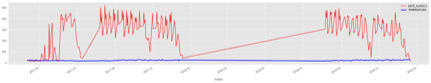
\includegraphics[width=\textwidth]{./Figuras/resultados/case1_temperatura.png}
                    	\caption{Correlação da distribuição do consumo com a temperatura.} \label{fig:case1_temperatura} }
                    \end{figure}\end{minipage} \hfill %
                      \begin{minipage}[c]{0.3\textwidth}
                \begin{figure}[H]
                	\center{                		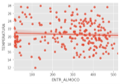
\includegraphics[width=\textwidth]{./Figuras/resultados/case1_temperatura_scatter.png}               	\caption{Gráfico scatter da distribuição do consumo com a temperatura.}
                	\label{fig:case1_temperatura_scatter_consumo} }   
                \end{figure}\end{minipage} \end{center} }
                
                
                %%%%%%%%%%%%%%%%%%%%%%%%%%%  UMIDADE   %%%%%%%%%%%%%%%%%%%%%%%%%%%%%%%%%%%%%%%%%%%%%%%%%
                 {\begin{center} \begin{minipage}[c]{0.6\textwidth}
                 \begin{figure}[H]
                    	\center{                    		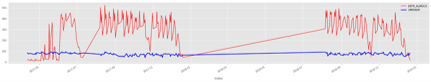
\includegraphics[width=\textwidth]{./Figuras/resultados/case1_umidade.png}
                    	\caption{Correlação da distribuição do consumo com a umidade.	} \label{fig:case1_umidade} }
                    \end{figure}
                    \end{minipage} \hfill %
                      \begin{minipage}[c]{0.3\textwidth}
                \begin{figure}[H]
                	\center{                		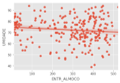
\includegraphics[width=\textwidth]{./Figuras/resultados/case1_umidade_scatter.png}
                	\caption{Gráfico scatter da distribuição do consumo com a umidade.}
                	\label{fig:case1_temperatura_scatter} }
                \end{figure}
                \end{minipage} \end{center} }
                
                
                %%%%%%%%%%%%%%%%%%%%%%%%%%%  VENTO   %%%%%%%%%%%%%%%%%%%%%%%%%%%%%%%%%%%%%%%%%%%%%%%%%
                {\begin{center} \begin{minipage}[c]{0.6\textwidth}
                 \begin{figure}[H]
                    	\center{                    		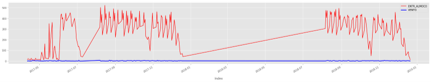
\includegraphics[width=\textwidth]{./Figuras/resultados/case1_vento.png}
                    	\caption{Correlação da distribuição do consumo com a velocidade do vento em m/s.} \label{fig:case1_vento} }
                    \end{figure}
                     \end{minipage} \hfill %
                      \begin{minipage}[c]{0.3\textwidth}
                    \begin{figure}[H]
                	\center{                		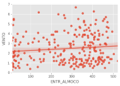
\includegraphics[width=\textwidth]{./Figuras/resultados/case1_vento_scatter.png}
                	\caption{Gráfico scatter da distribuição do consumo com a velocidade do vento.}
                \label{fig:case1_vento_scatter} }
                \end{figure}	
                \end{minipage} \end{center} }
                
                
                %%%%%%%%%%%%%%  PRESSAO ATMOSFERICA   %%%%%%%%%%%%%%%%%%%%%%%%%%%%%%%%%%%%%%%%%%%%%%%%%
                 
                 {\begin{center} \begin{minipage}[c]{0.6\textwidth}
                 \begin{figure}[H]
                    	\center{
                    		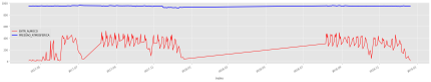
\includegraphics[width=\textwidth]{./Figuras/resultados/case1_pressao.png}
                    	\caption{Correlação da distribuição do consumo com a pressão atmosférica.} \label{fig:case1_pressao} }
                    \end{figure}
                        \end{minipage} \hfill %
                      \begin{minipage}[c]{0.3\textwidth}
                \begin{figure}[H]
                	\center{                		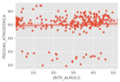
\includegraphics[width=\textwidth]{./Figuras/resultados/case1_pressao_scatter.png}
                	\caption{Gráfico scatter da distribuição do consumo com a pressão atmosférica.	} \label{fig:case1_pressao_scatter} }
                \end{figure}
                \end{minipage} \end{center} }
                
                
    	\subsection{Definição e treino dos modelos}
    	    Nesta seção os modelos de redes neurais foram desenvolvidos, treinados, avaliados sobre o conjunto de validação para obtermos métricas preliminares, e por fim foram testados.
    	    Na próxima subseção, 1 modelo inicial MLP é desenvolvido para avaliação da aprendizagem do problema.
    	    Como a avaliação de aprendizagem é um método comparativo com a profundidade em camadas do modelo, o mesmo modelo é redefinido com mais camadas de neurônios e novamente testado.
    	    Após os testes bem sucedidos sobre a avaliação de aprendizagem do problema nos modelos MLP, outros modelos com maior profundidade do tipo endógenos e exógenos foram desenvolvidos.
    	   % \newpage
    	    \subsubsection{Ajuste empírico de topologia com os modelos perceptron}
    	        %%%%%%%%%%%%%%%%%%%%% MLP 1 %%%%%%%%%%%%%%%%%%%%%%%%%%%%%%%%%%%%%%%%%%%
              \paragraph{MLP1}
    	        O primeiro modelo perceptron multilayer foi definido com uma camada de 15 unidades (mesmo número de features endógenas sendo 5 para consumo almoço , 5 para vendas de tickets e 5 para consumo de jantar, com intervalo de 5 dias).
    	        O modelo será denominado MLP1 para futuras referências. A figura abaixo foi obtida com o comando \textbf{keras.utils.plot\_model(MLP1, show\_shapes=True)}. Cada camada da rede corresponde à um bloco na figura, nos blocos são demonstrados o formato matricial dos parâmetros de  entrada. Nota-se que no primeiro bloco "InputLayer" são denotados o tamanho do intervalo temporal de cada parâmetro correspondente à 5 dias (de 1 dia anterior à 5 dias anteriores), e o número total de parâmetros que são 3 (ENTR\_ALMOCO, ENTR\_JANTAR e VENDAS\_ALMOCO).
    	        \begin{figure}[H]
                \center{
                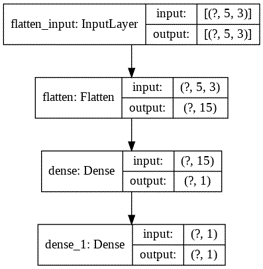
\includegraphics[width=0.5\textwidth]{./Figuras/resultados/case1_mlp1.png}
                	\caption{Topologia do modelo MLP1} 
                	\label{fig:case1_mlp1}
                }
                \end{figure}
                \begin{figure}[H]
                	\center{
                	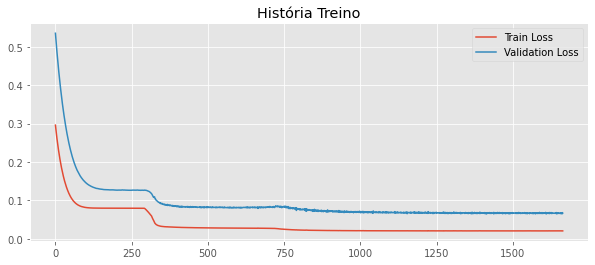
\includegraphics[width=0.8\textwidth]{./Figuras/resultados/case1_mlp1_train.png}
                	\caption{Gráfico de treino do modelo MLP1.}
                	\subcaption{Loss values, RMSE = 130.6207420543897}
                	\label{fig:case1_mlp1_train} 
                	}
                \end{figure}
    	        
    	        %%%%%%%%%%%%%%%%%%%%% MLP 2 %%%%%%%%%%%%%%%%%%%%%%%%%%%%%%%%%%%%%%%%%%%
    	        \paragraph{MLP2}
    	        Foi definido um novo modelo MLP2, aumentando o número de neurônios do MLP1 para a comparação do RMSE de treino.
    	        \begin{figure}[H]
                	\center{
                		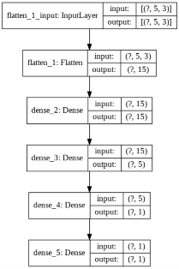
\includegraphics[width=0.3\textwidth]{./Figuras/resultados/case1_mlp2.png}
                	
                	\caption{Topologia do modelo MLP2} \label{fig:case1_mlp2} }
                \end{figure}
                \begin{figure}[H]
                	\center{
                		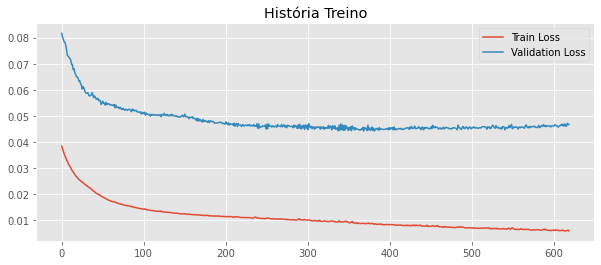
\includegraphics[width=1.0\textwidth]{./Figuras/resultados/case1_mlp2_train.png}
                
                	\caption{Gráfico de treino do modelo MLP2.	} 
                	\subcaption{RMSE = 107.97413966672336}
                	\label{fig:case1_mlp2_train} }
                \end{figure}
    	        É possível notar a diminuição do RMSE (Raiz do erro quadrático médio) ao aumentar a profundidade da rede perceptron para treino e avaliação sob o conjunto de validação. Validando a hipótese de que a predição do consumo no restaurante, pode ser aprendida por modelos simples de redes neurais, sendo possível avançar nas pesquisas com modelos que tragam melhores resultados.
    	    %%%%%%%%%%%%%%%%%%%%% MODELOS ENDÓGENOS ... VAMO LÁ ... TÁ ACABANDO ... %%%%%%%%%%%%%%%%%%%%%%%%%%%%%%%%%%%%%%%%%%%
          \subsubsection{Modelos Endógenos}
    	        Como o ajuste empírico obteve avanço nos resultados, foi definido outro modelo perceptron MLP\_ENDO\_1 com maior profundidade, e depois um modelo recorrente GRU com 2 reajustes (RNN\_ENDO\_1 e RNN\_ENDO\_2).
                Para a avaliação prévia dos modelos, os mesmos foram testados no conjunto de validação.\newline
    	        %%%%%%%%%%%%%%%%% MLP ENDO 1
              \paragraph{MLP\_ENDO\_1}
                Definido primeiro modelo endógeno exclusivamente perceptron, MLP\_ENDO\_1, com o aumento da profundidade de camadas de neurônios, baseado no modelo anterior MLP2.
      	        \begin{figure}[H]
                	\center{                		
                	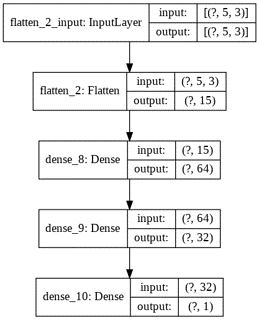
\includegraphics[width=0.5\textwidth]{./Figuras/resultados/case1_mlp_endo1.png}
                	\caption{Topologia do modelo MLP\_ENDO\_1} 
                	\label{fig:case1_mlp_endo1} 
                	}
                \end{figure}
                
               {
               \begin{center}
                    \begin{minipage}[c]{0.45\textwidth} 
                    \begin{figure}[H]
                      \center{
                        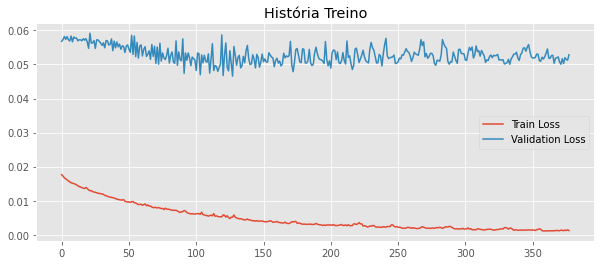
\includegraphics[width=\textwidth]{./Figuras/resultados/case1_mlp_endo1_train.png}
                        \caption{Treino do modelo MLP\_ENDO\_1} 
                        \label{fig:case1_mlp_endo1_train} 
                        }
                    \end{figure}  
                    \end{minipage} \hfill %
                    
                    \begin{minipage}[c]{1.0\textwidth}
                    \begin{figure}[H]
                      \center{
                        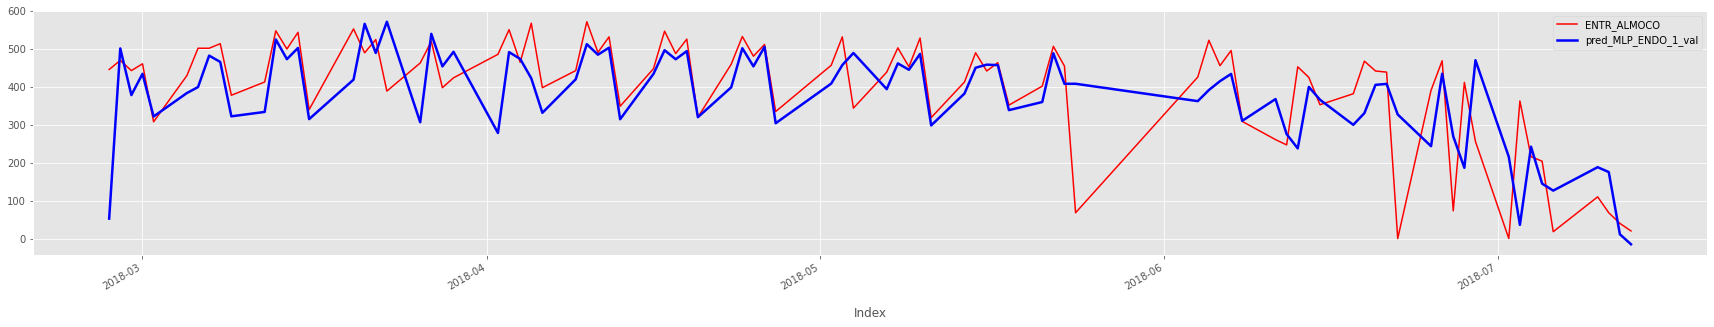
\includegraphics[width=\textwidth]{./Figuras/resultados/case1_mlp_endo1_val.png}
                        \caption{Avaliação do modelo MLP\_ENDO\_1} 
                        \label{fig:case1_mlp_endo1_val} 
                        }
                    \end{figure}
                    \end{minipage} 
                \end{center} 
                }
                
                \begin{table}[!ht]
                \centering
                \rowcolors{2}{gray!25}{white}
                \begin{tabular}{|c|c|}
                \hline
                \multicolumn{2}{c}{METRICAS DO MODELO MLP\_ENDO\_1 :}\\ \hline
                RMSE &  110.92902359567118\\
                TOTAL DE REFEIÇÕES PROJETADAS & 89 : 33611.37430477142\\
                TOTAL DE REFEIÇÕES CONSUMIDAS & 89 : 35555\\
                TOTAL DE REFEIÇÕES SUB PROJETADAS & -4328.862397193909\\
                TOTAL DE REFEIÇÕES SUPER PROJETADAS & 2385.236701965332\\
                \hline
                \end{tabular} 
                \caption{Métricas de avaliação do modelo MLP\_ENDO\_1.}
                \label{table:case1_mlp_endo1_val_table}
                \end{table}
                 
              %%%%%%%%%%%%%%%%% RNN ENDO 1
              
              \paragraph{RNN\_ENDO\_1}
               Definido primeiro modelo com a utilização das redes recorrentes GRU, RNN\_ENDO\_1, para comparação de resultados com o modelo anterior perceptron.
                \begin{figure}[H]
                  \center{
                    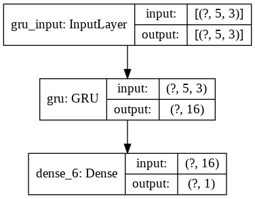
\includegraphics[width=0.6\textwidth]{./Figuras/resultados/case1_rnn_endo1.png}
                  \caption{Topologia do modelo RNN\_ENDO\_1} \label{fig:case1_rnn_endo1} }
                \end{figure}

                {
                \begin{center}
                    \begin{minipage}[c]{0.5\textwidth}
                    \begin{figure}[H]
                      \center{
                        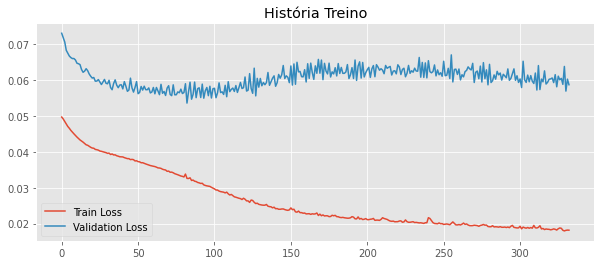
\includegraphics[width=\textwidth]{./Figuras/resultados/case1_rnn_endo1_train.png}
                      \caption{Treino do modelo RNN\_ENDO\_1} 
                      \label{fig:case1_rnn_endo1_train} 
                      }
                    \end{figure} 
                    \end{minipage} \hfill %
                    
                    \begin{minipage}[c]{1.0\textwidth}
                    \begin{figure}[H]
                      \center{
                        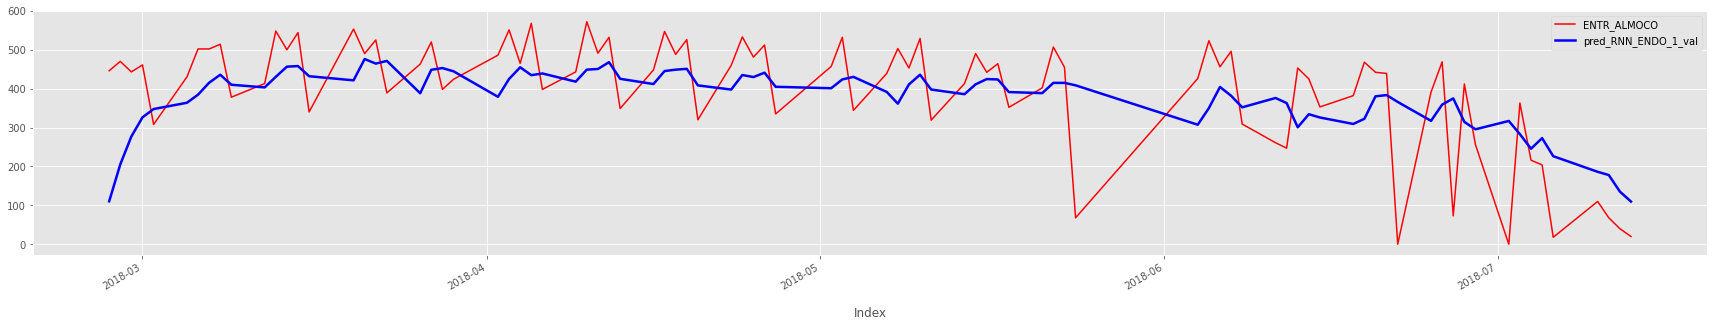
\includegraphics[width=\textwidth]{./Figuras/resultados/case1_rnn_endo1_val.png}
                      \caption{Avaliação do modelo RNN\_ENDO\_1} \label{fig:case1_rnn_endo1_val} }
                    \end{figure}
                    \end{minipage} 
                \end{center} 
                }
                
                \begin{table}[!ht]
                   \centering
                   \caption{Métricas de avaliação do modelo RNN\_ENDO\_1.}
                 \rowcolors{2}{gray!25}{white}
                \begin{tabular}{|c|c|}
                \rowcolor{gray!50} \hline
                \multicolumn{2}{c}{ METRICAS DO MODELO RNN\_ENDO\_1 : }\\ \hline
                RMSE & 118.98273426840373\\
                TOTAL DE REFEIÇÕES PROJETADAS & 33423.96739196777\\
                TOTAL DE REFEIÇÕES CONSUMIDAS & 35555\\
                TOTAL DE REFEIÇÕES SUB PROJETADAS & -5248.0078125\\
                TOTAL DE REFEIÇÕES SUPER PROJETADAS & 3116.9752044677734\\
                \hline
                \end{tabular}\end{table}

            %%%%%%%%%%%%%%%%% RNN ENDO 2
             \paragraph{RNN\_ENDO\_2}
                Definido segundo modelo GRU, RNN\_ENDO\_2, com o aumento da profundidade de unidades do modelo anterior RNN\_ENDO\_1 e com a inclusão do recurso Dropout para eliminar unidades com pesos negativos no grafo denso da rede, realizando a poda de unidades não relevantes.
                \begin{figure}[H]
                  \center{
                    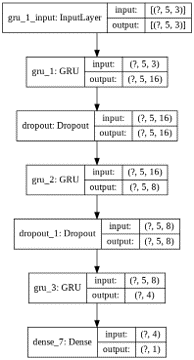
\includegraphics[width=0.4\textwidth]{./Figuras/resultados/case1_rnn_endo2.png}
                  
                  \caption{Topologia do modelo RNN\_ENDO\_2} \label{fig:case1_rnn_endo2} }
                \end{figure}
        {\begin{center} \begin{minipage}[c]{0.45\textwidth}
                \begin{figure}[H]
                  \center{
                    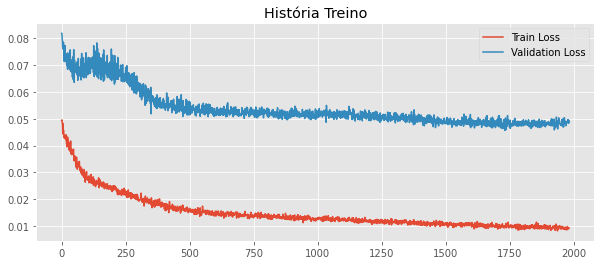
\includegraphics[width=\textwidth]{./Figuras/resultados/case1_rnn_endo2_train.png}
                  \caption{Treino do modelo RNN\_ENDO\_2} \label{fig:case1_rnn_endo2_train} }
                \end{figure}\end{minipage} \hfill %
                      \begin{minipage}[c]{1.0\textwidth}
                \begin{figure}[H]
                  \center{
                    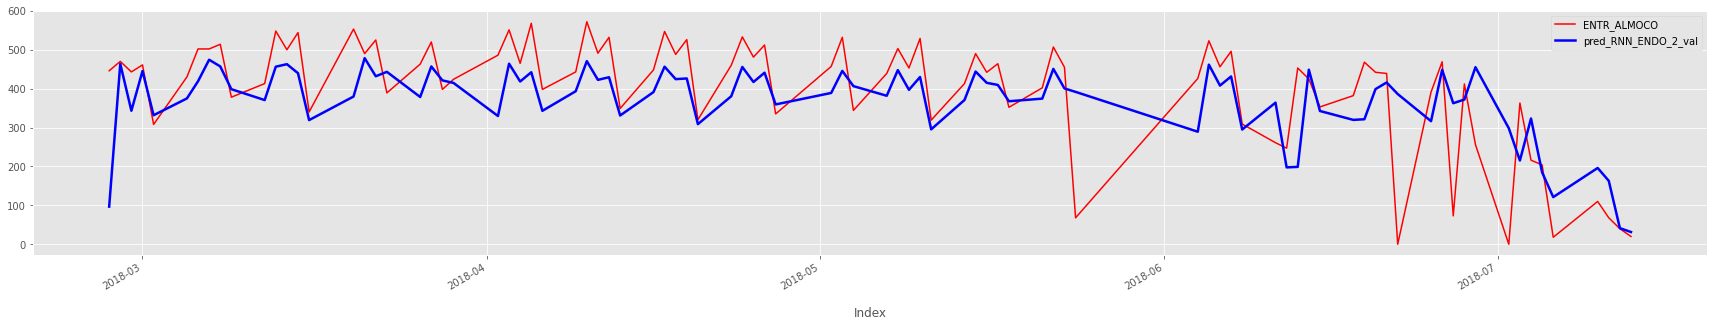
\includegraphics[width=\textwidth]{./Figuras/resultados/case1_rnn_endo2_val.png}
                  \caption{Avaliação do modelo RNN\_ENDO\_2} \label{fig:case1_rnn_endo2_val} }
                \end{figure}
                 \end{minipage} \end{center} }
                
                   \begin{table}[!ht]
                   \centering
                   \caption{Métricas de avaliação do modelo RNN\_ENDO\_2 }
                \rowcolors{2}{gray!25}{white}
                    \begin{tabular}{|c|c|}
                    \rowcolor{gray!50}
                    \hline
                \multicolumn{2}{c}{METRICAS DO MODELO RNN\_ENDO\_2 :}  \\ \hline
                RMSE & 109.81020024143946\\
                TOTAL DE REFEIÇÕES PROJETADAS & 32984.970529556274\\
                TOTAL DE REFEIÇÕES CONSUMIDAS & 35555\\
                TOTAL DE REFEIÇÕES SUB PROJETADAS & -4821.583518981934\\
                TOTAL DE REFEIÇÕES SUPER PROJETADAS & 2251.554048538208\\
                \hline \end{tabular} \end{table}
                
                % \newpage
                \paragraph{Comparativo gráfico da etapa de avaliação entre RNN\_ENDO\_2 e MLP\_ENDO\_1}
                
                  É possível notar, conforme figura \ref{fig:case1_gru_mlp_val_analise} que mesmo com correlação e RMSE muito próximo nos 2 modelos, o modelo RNN\_ENDO\_2 apresentou melhor valor p-value, no calculo de correlação de Pearson*. 
                  Em Junho após uma ocorrência outlier, o modelo GRU teve melhor recuperação de resultados em comparação ao MLP.
                  De acordo com a referência da documentação da biblioteca scipy, o valor p-value indica aproximadamente a probabilidade de um sistema não correlacionado produzir conjuntos de dados que têm uma correlação de Pearson pelo menos tão extrema quanto a calculada a partir desses conjuntos de dados.\newline.
                  Podemos notar também que o recurso dropout realizou a poda de unidades de forma bem sucedida gerando melhores resultados, em comparação ao modelo RNN\_ENDO\_1 sem a poda.
                    
                %   \newpage
                  RNN\_ENDO\_2 :\newline 
                  CORRELAÇÃO (r): 0.6753384458677313 \newline
                  Pi (p) :3.903678433027079e-13
                  
                  MLP\_ENDO\_1 :\newline 
                  MLP: CORRELAÇÃO (r): 0.6791684214084684 \newline
                  Pi (p) :2.5590689588089596e-13\newline
                  \begin{figure}[H]
                      \center{
                        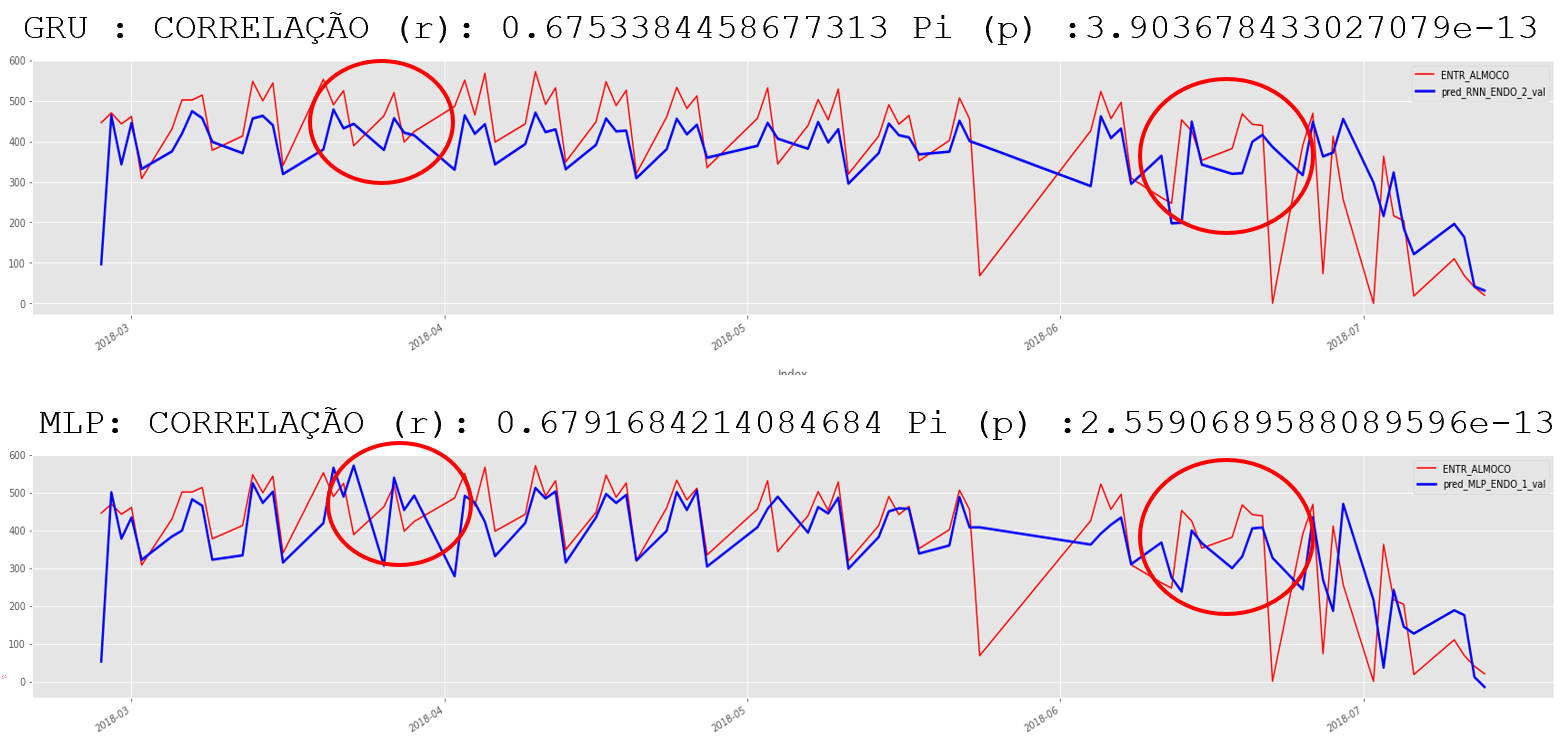
\includegraphics[width=1.0\textwidth]{./Figuras/resultados/case1_gru_mlp_val_analise.PNG}
                      \caption{Comparação da etapa de validação entre MLP\_ENDO\_1 e RNN\_ENDO\_1} \label{fig:case1_gru_mlp_val_analise} }
                    \end{figure}

          %%%%%%%%%%%%%%%%%%%%% MODELOS EXÓGENOS ... 2 DA MANHÃ... Q Q EU FUI INVENTAR NESSE TRABALHO ... %%%%%%%%%%%%%%%%%%%%%%%%%%%%%%%%%%%%%%%%%%%
            % \newpage
            
    	    \subsubsection{Modelos mistos endógenos e exógenos}
    	    Nos modelos desta subseção, a coluna de blocos à esquerda na figura de topologia do modelo, trata as entradas endógenas (temporais) com camadas GRU. A coluna à direita trata as entradas exógenas como variáveis climáticas e de calendário com camadas do tipo MLP.
    	    A saída de ambas as distintas camadas é concatenada e tratada por uma camada MLP de saída.
            %%%%%%%%%%%%%%%%% RNN_EXO_1
              \paragraph{RNN\_EXO\_1} Primeiro modelo misto, com camada GRU à esquerda e MLP à direita.
                \begin{figure}[H]
                  \center{
                    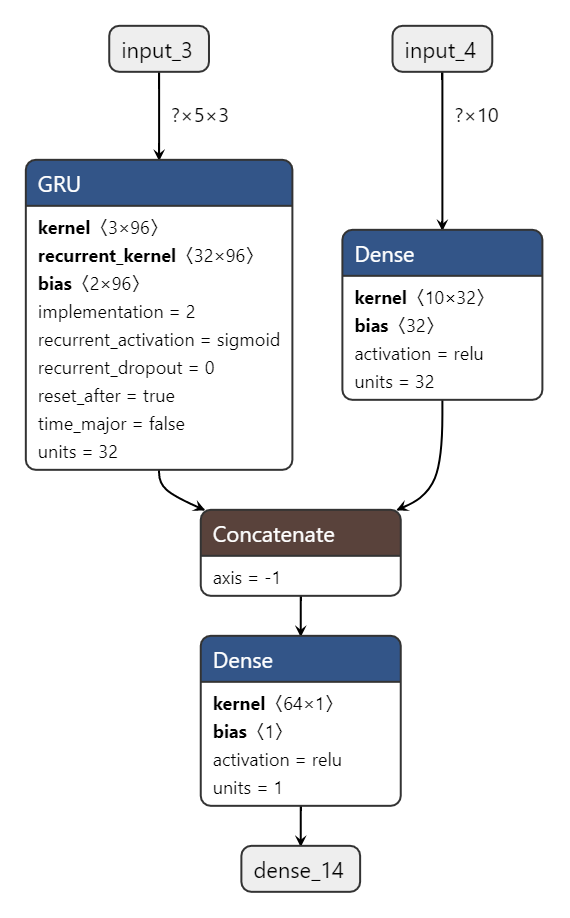
\includegraphics[width=0.7\textwidth]{./Figuras/resultados/case1_rnn_exo_1.png}
                  
                  \caption{Topologia do modelo RNN\_EXO\_1} \label{fig:case1_rnn_exo_1} }
                \end{figure}

                {\begin{center} \begin{minipage}[c]{0.45\textwidth}
                \begin{figure}[H]
                  \center{                    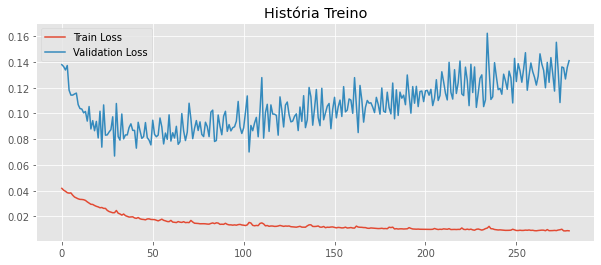
\includegraphics[width=\textwidth]{./Figuras/resultados/case1_rnn_exo_1_train.png}
                  \caption{Treino do modelo RNN\_EXO\_1} \label{fig:case1_rnn_exo_1_train} }
                \end{figure}
                \end{minipage} \hfill %
                      \begin{minipage}[c]{1.0\textwidth}
                \begin{figure}[H]
                  \center{                    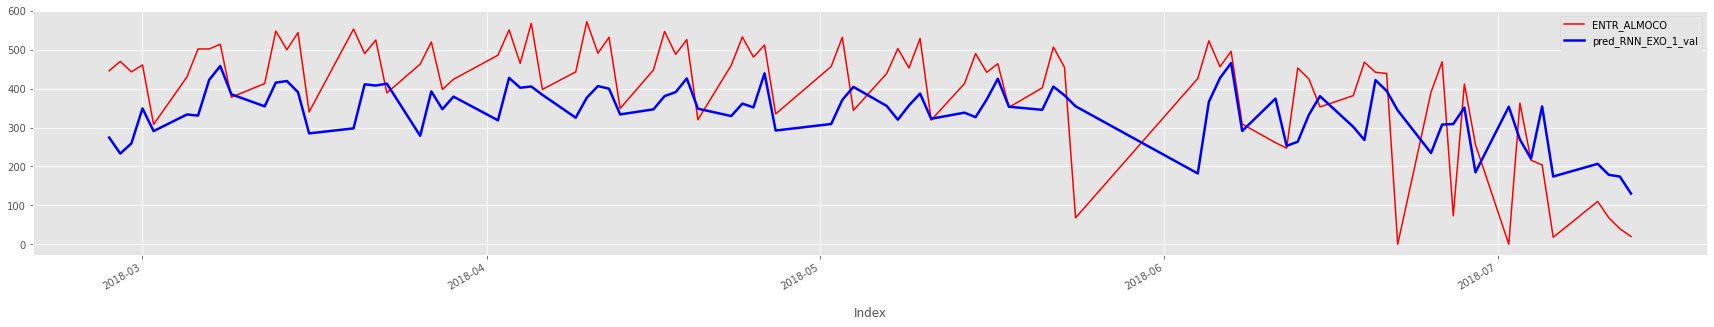
\includegraphics[width=\textwidth]{./Figuras/resultados/case1_rnn_exo_1_val.png}
                    \caption{Avaliação do modelo RNN\_EXO\_1} \label{fig:case1_rnn_exo_1_val} }
                \end{figure}                
                \end{minipage}
                     \begin{minipage}[c]{0.45\textwidth}
                  \begin{figure}[H]
                  \center{                    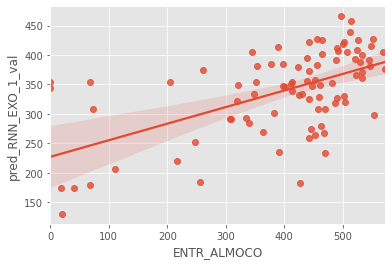
\includegraphics[width=\textwidth]{./Figuras/resultados/case1_rnn_exo_1_val_scatter.png}
                    \caption{Grafico scatter de avaliação do modelo RNN\_EXO\_1} \label{fig:case1_rnn_exo_1_val_scatter} }
                \end{figure}
                \end{minipage} \end{center} }
               
                
                \begin{table}[!ht]
                \centering
                \caption{Métricas do modelo  RNN\_EXO\_1 }
                \rowcolors{2}{gray!25}{white}
                \begin{tabular}{|c|c|}
                \rowcolor{gray!50}
                \hline
                \multicolumn{2}{c}{METRICAS DO MODELO RNN\_EXO\_1 :}\\ \hline
                RMSE & 132.9496\\
                TOTAL DE REFEIÇÕES PROJETADAS & 30223.764709472656\\
                TOTAL DE REFEIÇÕES CONSUMIDAS & 35555\\
                TOTAL DE REFEIÇÕES SUB PROJETADAS & -7585.754409790039\\
                TOTAL DE REFEIÇÕES SUPER PROJETADAS & 2254.5191192626953\\
                \hline \end{tabular} \end{table}
                % \newpage
                
              %%%%%%%%%%%%%%%%% RNN_EXO_2
              \paragraph{RNN\_EXO\_2} Segundo modelo misto definido com o aumento da profundidade das camadas GRU e MLP do modelo anterior.
                \begin{figure}[H]
                  \center{
                    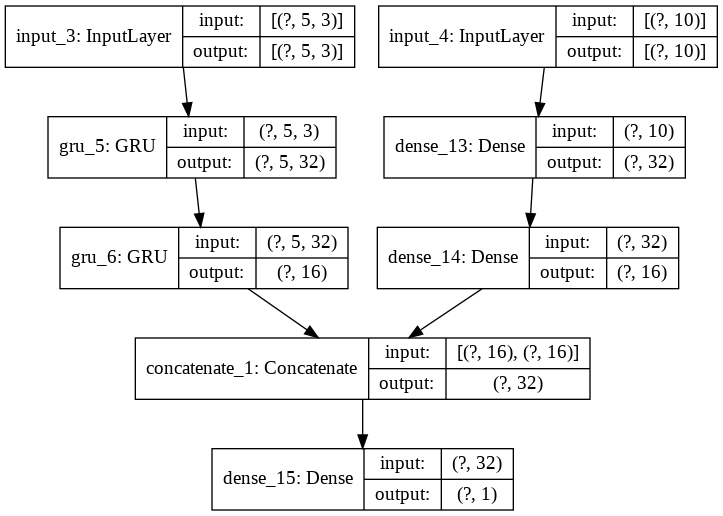
\includegraphics[width=0.7\textwidth]{./Figuras/resultados/case1_rnn_exo_2.png}
                 
                  \caption{Topologia do modelo RNN\_EXO\_2}  \label{fig:case1_rnn_exo_2} }
                \end{figure}
                
            {\begin{center} \begin{minipage}[c]{0.45\textwidth}
                \begin{figure}[H]
                  \center{                    \includegraphics[width=\textwidth]{./Figuras/resultados/case1_rnn_exo_2_train.png}
                  \caption{Treino do modelo RNN\_EXO\_2} \label{fig:case1_rnn_exo_2_train} }
                \end{figure}\end{minipage} \hfill %
                  \begin{minipage}[c]{1.0\textwidth}
                \begin{figure}[H]
                  \center{                    \includegraphics[width=\textwidth]{./Figuras/resultados/case1_rnn_exo_2_val.png} 
                  \caption{Avaliação do modelo RNN\_EXO\_2} \label{fig:case1_rnn_exo_2_val} }
                  \end{figure}  
                     \end{minipage}
                     \begin{minipage}[c]{0.45\textwidth}
                  \begin{figure}[H]
                  \center{                   \includegraphics[width=\textwidth]{./Figuras/resultados/case1_rnn_exo_2_val_scatter.png} }
                  \caption{Grafico scatter de avaliação do modelo RNN\_EXO\_2 \label{fig:case1_rnn_exo_2_val_scatter} }
                \end{figure}
                  \end{minipage} \end{center} }
                
                
               
                
                 \begin{table}[!ht]
                \centering
                \caption{Métricas do modelo  RNN\_EXO\_2 }
                \rowcolors{2}{gray!25}{white}
                 \begin{tabular}{|c|c|}
                 \rowcolor{gray!50}
                 \hline
                \multicolumn{2}{c}{METRICAS DO MODELO RNN\_EXO\_2 :}\\ \hline
                RMSE & 122.32142544582184\\
                TOTAL DE REFEIÇÕES PROJETADAS & 32146.112915039062\\
                TOTAL DE REFEIÇÕES CONSUMIDAS & 35555\\
                TOTAL DE REFEIÇÕES SUB PROJETADAS & -5875.795913696289\\
                TOTAL DE REFEIÇÕES SUPER PROJETADAS & 2466.9088287353516\\
                \hline \end{tabular}
                \end{table}
                
            %  \newpage   
                
          %%%%%%%%%%%%%%%%% RNN_EXO_3
              \paragraph{RNN\_EXO\_3}
                Terceiro modelo misto, com a utilização de dropout na camada GRU baseada no melhor modelo endógeno RNN\_ENDO\_2, mantendo a camanda MLP à direita sem alterações.
              
                \begin{figure}[H]
                  \center{
                    \includegraphics[width=1.0\textwidth]{./Figuras/resultados/case1_rnn_exo_3.png}
                  
                  \caption{Topologia do modelo RNN\_EXO\_3} \label{fig:case1_rnn_exo_3} }
                \end{figure}

                {\begin{center} \begin{minipage}[b]{0.45\textwidth}
                \begin{figure}[H]
                  \center{                    \includegraphics[width=\textwidth]{./Figuras/resultados/case1_rnn_exo_3_train.png}
                  \caption{Treino do modelo RNN\_EXO\_3} \label{fig:case1_rnn_exo_3_train} }
                \end{figure}\end{minipage} \hfill %
                      \begin{minipage}[b]{1.0\textwidth}
                \begin{figure}[H]
                  \center{                    \includegraphics[width=\textwidth]{./Figuras/resultados/case1_rnn_exo_3_val.png}
                  \caption{Avaliação do modelo RNN\_EXO\_3} \label{fig:case1_rnn_exo_3_val} }
                \end{figure}  \end{minipage} 
                \begin{minipage}[b]{0.45\textwidth}
                \begin{figure}[H]
                  \center{                    \includegraphics[width=\textwidth]{./Figuras/resultados/case1_rnn_exo_3_val_scatter.png}
                  }
                  \caption{Grafico scatter de avaliação do modelo RNN\_EXO\_3 \label{fig:case1_rnn_exo_3_val_scatter} }
                \end{figure} \end{minipage}
                \end{center} }
                
                
                
                
                
                 \begin{table}[!ht]
                \centering
                \caption{Métricas do modelo  RNN\_EXO\_3 }
                   \rowcolors{2}{gray!25}{white}
                 \begin{tabular}{|c|c|}
                     \rowcolor{gray!50}
                     \hline
                     \multicolumn{2}{c}{ METRICAS DO MODELO RNN\_EXO\_3 : } \\ \hline
                        RMSE & 121.25903250027721\\
                        TOTAL DE REFEIÇÕES PROJETADAS & 35003.56196594238\\
                        TOTAL DE REFEIÇÕES CONSUMIDAS &  35555\\
                        TOTAL DE REFEIÇÕES SUB PROJETADAS & -4471.480010986328\\
                        TOTAL DE REFEIÇÕES SUPER PROJETADAS & 3920.041976928711 \\ \hline 
                \end{tabular} \end{table}
        % \newpage
        
    	\subsection{Teste e métricas}
    	    Nesta subseção todos os modelos foram testados no conjunto de teste, 1o semestre de 2019. Em práticas com maior volume de modelos, pode-se selecionar apenas os modelos com os melhores resultados na etapa de validação. Porém, para um número de 6 modelos foi considerado o teste em todos os modelos a fim de documentação dos resultados em proveito à trabalhos futuros. 
    	    Entre todos os 6 modelos, é selecionado o melhor modelo endógeno, o melhor exógeno, e ambos foram selecionados para comparações com a fase 2.
    	    
    	    \subsubsection{Endógenos : GRU x MLP}
    	    
            \begin{table}[!ht]
            \centering
            \rowcolors{2}{gray!25}{white}
            \begin{tabular}{|c|c|c|c|}
            \rowcolor{gray!50}
            \hline
                Modelo &  Correlação & P-value & RMSE: \\ \hline
                RNN\_ENDO\_2 & 0.5954398951050144 & 9.422151772316392e-10 & 108.0662\\ 
                 MLP\_ENDO\_1 & 0.5212411617024483 & 1.9211576129056944e-07 & 128.0541\\
            \hline 
            \end{tabular}
            \caption{Métricas dos melhores modelos RNN\_ENDO\_2 x MLP\_ENDO\_1}
            \label{table:case1_GRUvsMLP}
            \end{table}
            
            {\begin{center} \begin{minipage}[b]{1.0\textwidth}
            \begin{figure}[H]
              \center{
                \includegraphics[width=\textwidth]{./Figuras/resultados/case1_mlp_endo1_test.png}
              \caption{Teste MLP\_ENDO\_1} \label{fig:case1_mlp_endo1_test} }
            \end{figure}\end{minipage} \hfill %
                      \begin{minipage}[b]{1.0\textwidth}
            \begin{figure}[H]
              \center{
                \includegraphics[width=\textwidth]{./Figuras/resultados/case1_rnn_endo2_test.png}
              \caption{Teste RNN\_ENDO\_2} \label{fig:case1_rnn_endo2_test} }
            \end{figure} \end{minipage} \end{center} }
            
            Podemos notar na figura \ref{fig:case1_mlp_endo1_test} e \ref{fig:case1_rnn_endo2_test} que apesar dos coeficientes de correlação serem próximos no teste entre os modelos RNN\_ENDO\_2 e MLP\_ENDO\_1, as métricas da tabela \ref{table:case1_GRUvsMLP} para o valor p-value e RMSE (métrica utilizada no treino dos modelos) é discrepante e seleciona o modelo GRU como o melhor modelo nesta comparação.\newline

    	    \subsubsection{Melhor modelo Endógeno}
            De acordo com as métricas de teste, o melhor modelo endógeno foi o RNN\_ENDO\_2, e suas anomalias de previsão foram devidamente justificadas por datas especiais no calendário do primeiro semestre:
            
            \begin{figure}[H]
              \center{
                \includegraphics[width=1.0\textwidth]{./Figuras/resultados/case1_rnn_endo2_test_dates.png}
              \caption{Analise de anomalias preditivas do RNN\_ENDO\_2} \label{fig:case1_rnn_endo2_test_dates} }
            \end{figure}
            
            As datas que produziram outliers e anomalias de predição no melhor modelo endógeno, podem ser observadas na figura \ref{fig:case1_rnn_endo2_test_dates}, sendo os pontos verdes outliers onde o modelo seguiu a tendência de alta ou baixa de consumo mas obteve erro discrepante, e nos pontos vermelhos seguiu tendência inversa:

            \begin{table}[!ht]
                \centering
                \rowcolors{2}{gray!25}{white}
                 \begin{tabular}{|c|c|c|}
                 \rowcolor{gray!50}
                 \hline 
             Data & Consumo & Justificativa\\ \hline    
            01/03/2019 (sexta feira)    & 224 & Sexta Feira pré - carnaval\\
             03/06/2019 (segunda feira)  &  13 & Segunda Feira pós paralisação estudantil\\ \hline \end{tabular} \end{table}

            Datas com anomalias de previsão onde o modelo seguiu tendência oposta ao consumo, pontos vermelhos:
            \begin{table}[!ht]
                \rowcolors{2}{gray!25}{white}
                 \begin{tabular}{|c|c|c|}
                 \rowcolor{gray!50}
                 \hline
            Data & Consumo & Justificativa \\
            08/03/2019 (sexta feira)   & 209 &Sexta Feira pós - carnaval\\
           15/05/2019 (quarta feira)   & 19  & Paralisação estudantil na praça Afonso Pena\\
            30/05/2019 (quinta feira)   &  38  & Paralisação estudantil na Praça Afonso pena\\
            \hline \end{tabular} \end{table}

            Métricas do melhor modelo: 
            \begin{table}[!ht]
            \centering
            \rowcolors{2}{gray!25}{white}
            \begin{tabular}{|c|c|}
            \rowcolor{gray!50}
            \hline
                Melhor modelo: &   RNN\_ENDO\_2: \\ \hline
                Total\_Consumidas & 31962 \\ 
                Total\_Previstas & 31465,61133 \\
                Erro\_Total\_Previsao & -496,3886719 \\
                Percentual\_Erro\_Total & -1,5530\% \\\
                Correlação & 0,595439895 \\
                P-value & 9,42215E-10    \\
                RMSE &  108,0663015\\
                Total de Refeições em falta & -2982,567947 \\Total Descartadas & 3478,957266\\
                ERRO\_ABS\_MEDIANO & 46,70721436 
                \\ ERRO\_ABSOLUTO\_PERCENTUAL\_MEDIO & 74,93539002 \\ 
            \hline 
            \end{tabular}
            \caption{Métricas do melhor modelo:  RNN\_ENDO\_2 }
            \label{table:rnn_endo_2_test}
            \end{table}
            
                 \begin{figure}[H]
              \center{
                \includegraphics[width=0.5\textwidth]{./Figuras/resultados/case1_rnn_endo2_test_scatter.png}
              \caption{Grafico scatter de teste do RNN\_ENDO\_2} \label{fig:case1_rnn_endo2_test_scatter} }
            \end{figure}
            
    	    \subsubsection{Modelos mistos}
    	       Todos os modelos mistos compõem uma mesma classe, que combina camadas GRU com MLP, portanto as métricas são registradas à seguir, por paragrafo, para cada modelo. Diferentemente nos endógenos onde haviam 2 modelos GRU e 1 MLP compondo classes diferentes e sendo necessário um paragrafo extra de comparação entre o melhor GRU e o MLP.
    	       Os parágrafos a seguir apenas reúnem todas as informações entre os modelos para extrair o melhor modelo com a melhor métrica de RMSE.
    	    
    	   % \newpage
    	     %%%%%%%%%%%%%%%%% RNN_EXO\_1
    	     \paragraph{RNN\_EXO\_1}
        	    {
        	    \begin{center} 
        	        \begin{minipage}[c]{1.0\textwidth}
                      \begin{figure}[H]
                          \center{                    \includegraphics[width=\textwidth]{./Figuras/resultados/case1_rnn_exo_1_test.png}
                          \caption{Teste do modelo RNN\_EXO\_1} 
                          \label{fig:case1_rnn_exo_1_test} }
                        \end{figure} 
                    \end{minipage} \hfill %
                    
                    \begin{minipage}[c]{0.5\textwidth}
                        \begin{figure}[H]
                          \center{                    \includegraphics[width=\textwidth]{./Figuras/resultados/case1_rnn_exo_1_test_scatter.png}
                            \caption{Grafico scatter de teste do modelo RNN\_EXO\_1} \label{fig:case1_rnn_exo_1_test_scatter} }
                            \end{figure}
                    \end{minipage} 
                \end{center} }
                
                \begin{table}[!ht]
                \centering
                \caption{Erros do modelo  RNN\_EXO\_1 }
                \rowcolors{2}{gray!25}{white}
                    \begin{tabular}{|c|c|}
                    \rowcolor{gray!50}
                    \hline
                \multicolumn{2}{c}{RNN\_EXO\_1:} \\
                \hline
                TOTAL DE REFEIÇÕES CONSUMIDAS & 31962 : 88  \\
                TOTAL DE REFEIÇÕES PROJETADAS & 28728.816 : 88  \\
                ERRO DE PREVISÃO & -3233.18359375 \\
                PERCENTAGEM DE ERRO & -10.115711137444466\%  \\
                CORRELAÇÃO (r) & 0.4122158648305426 \\ Pi (p) & 6.590759241637016e-05\\ R2 & 0.16992191921799218\\
                RMSE & 124.49076120428357\\
                ERRO TOTAL DE REFEIÇÕES SUB PROJETADAS & -2709.1732788085938\\
                ERRO TOTAL DE REFEIÇÕES SUPER PROJETADAS & 5942.356475830078\\
                ERRO ABSOLUTO MEDIANO & 85.59107971191406\\
                ERRO ABSOLUTO PERCENTUAL MEDIO & 90.98694558104974\% \\ \hline \end{tabular} \end{table}
                
        % \newpage
        \paragraph{RNN\_EXO\_2}
        {\begin{center} \begin{minipage}[c]{1.0\textwidth}
             %%%%%%%%%%%%%%%%% RNN_EXO_2
                \begin{figure}[H]
                  \center{                \includegraphics[width=\textwidth]{./Figuras/resultados/case1_rnn_exo_2_test.png}
                  \caption{Teste do modelo RNN\_EXO\_2} \label{fig:case1_rnn_exo_2_test} }
                \end{figure}\end{minipage} \hfill %
                      \begin{minipage}[c]{0.5\textwidth}
                \begin{figure}[H]
                  \center{                    \includegraphics[width=\textwidth]{./Figuras/resultados/case1_rnn_exo_2_test_scatter.png}
                  \caption{Grafico scatter de teste do modelo RNN\_EXO\_2} \label{fig:case1_rnn_exo_2_test_scatter} }
                \end{figure}
                \end{minipage} \end{center} }
               
                \begin{table}[!ht]
                \centering
                \caption{Erros do modelo  RNN\_EXO\_2 } 
                \rowcolors{2}{gray!25}{white}
                    \begin{tabular}{|c|c|}
                    \rowcolor{gray!50}
                    \hline
                \multicolumn{2}{c}{RNN\_EXO\_2:} \\ \hline
                TOTAL DE REFEIÇÕES CONSUMIDAS & 31962 : 88 \\
                TOTAL DE REFEIÇÕES PROJETADAS & 30823.148 : 88 \\
                ERRO DE PREVISÃO & -1138.8515625 \\
                PERCENTAGEM DE ERRO &  -3.563142364370189 \\
                CORRELAÇÃO (r)& 0.5206433612135913\\ Pi (p) & 1.995208420251518e-07\\
                R2 & 0.27106950957578635\\
                RMSE & 112.99211377165491\\
                ERRO TOTAL DE REFEIÇÕES SUB PROJETADAS & -3044.8834533691406\\
                ERRO TOTAL DE REFEIÇÕES SUPER PROJETADAS & 4183.734128952026\\
                ERRO ABSOLUTO MEDIANO & 63.59894561767578\\
                ERRO ABSOLUTO PERCENTUAL MEDIO & 88.26875085831726\% \\ \hline \end{tabular}\end{table}
                
              
             %%%%%%%%%%%%%%%%% RNN_EXO_3
            %   \newpage
              \paragraph{RNN\_EXO\_3}
                \begin{figure}[H]
                  \center{
                    \includegraphics[width=1.0\textwidth]{./Figuras/resultados/case1_rnn_exo_3_test.png}
                  
                  \caption{Teste do modelo RNN\_EXO\_3} \label{fig:case1_rnn_exo_3_test} }
                \end{figure}

                \begin{figure}[H]
                  \center{
                    \includegraphics[width=0.7\textwidth]{./Figuras/resultados/case1_rnn_exo_3_test_scatter.png}
                  
                  \caption{Grafico scatter de teste do modelo RNN\_EXO\_3} \label{fig:case1_rnn_exo_3_test_scatter} }
                \end{figure}
                
                 \begin{table}[!ht]
                \centering
                \caption{Erros do modelo  RNN\_EXO\_3 }
                \rowcolors{2}{gray!25}{white}
                    \begin{tabular}{|c|c|}
                    \rowcolor{gray!50}
                    \hline
               \multicolumn{2}{c}{ RNN\_EXO\_3:} \\ \hline
                TOTAL DE REFEIÇÕES CONSUMIDAS & 31962 : 88 \\
                TOTAL DE REFEIÇÕES PROJETADAS  & 29425.791 : 88 \\
                ERRO DE PREVISÃO\ -2536.208984375\\ 
                PERCENTAGEM DE ERRO &-7.935075978896815\% \\
                CORRELAÇÃO (r) & 0.33963283016931 \\ Pi (p)& 0.0012067360859947137 \\R2 & 0.11535045932881538\\
                RMSE & 124.65810037942255\\
                ERRO TOTAL DE REFEIÇÕES SUB PROJETADAS & -3417.6602630615234\\
                ERRO TOTAL DE REFEIÇÕES SUPER PROJETADAS & 5953.868759155273\\
                ERRO ABSOLUTO MEDIANO & 100.44429016113281\\
                ERRO ABSOLUTO PERCENTUAL MEDIO & 98.79064922123037\% \\ \hline \end{tabular} \end{table}
            
            % \newpage
    	    \subsection{Melhor modelo da 1a fase}
                Entre todos os modelos, o melhor modelo produzindo o menor RMSE e com vantagem em todas as outras métricas foi o modelo endógeno, RNN\_ENDO\_2, ressaltando que o gráfico e as métricas de predições deste modelo se encontram na figura \ref{fig:case1_rnn_endo2_test}.
                Na ultima seção deste capítulo são apresentadas todas as métricas de todos os modelos de todas as fases experimentais.

    \section{Fase Experimental II}
        
        \begin{figure}[H]
        	\center{
        		\includegraphics[width=1.0\textwidth]{./Figuras/resultados/case2/case2_dominio.png}
        	
        	\caption{Domínio temporal da 2a fase} \label{fig:case2_timeline} }
        \end{figure}
	    Nesta segunda fase, todos os modelos da fase anterior foram importados, treinados e testados sobre um novo domínio temporal de acordo com a figura \ref{fig:case2_timeline}.
        
        % \newpage
	    \subsection{Pré-Processamento}
	        Nesta subseção para a etapa de pré-processamento foram avaliados apenas os resultados obtidos da divisão dos conjuntos e da técnica aplicada do restaurante.
	        
    	    \paragraph{Divisão dos conjuntos}
    	    {\begin{center} \begin{minipage}[b]{0.45\textwidth}
    	        %%% TREINO
    	        \begin{figure}[H]
                  \center{                    \includegraphics[width=\textwidth]{./Figuras/resultados/case2/case2_train.png}
                  \caption{Conjunto de dados de treino, ano de 2017 completo} \label{fig:case2_train} }
                \end{figure}
                \end{minipage} \hfill %
                 \begin{minipage}[b]{0.45\textwidth}
                %%% VALIDAÇÃO
                \begin{figure}[H]
                  \center{                    \includegraphics[width=\textwidth]{./Figuras/resultados/case2/case2_val.png}
                  \caption{Conjunto de dados de validação, ano de 2018 completo} \label{fig:case2_val} }
                \end{figure}
                \end{minipage}
                 \begin{minipage}[b]{0.45\textwidth}
                %%% TESTE
                \begin{figure}[H]
                  \center{                  \includegraphics[width=\textwidth]{./Figuras/resultados/case2/case2_test.png}
                  \caption{Conjunto de dados de teste, ano de 2019 completo} \label{fig:case2_test} }
                \end{figure}
                \end{minipage} \end{center} }
    	        
    	        A nova divisão dos conjuntos segue conforme as figuras \ref{fig:case2_train} para o conjunto de treino, \ref{fig:case2_train} para o conjunto de validação e \ref{fig:case2_train} para o conjunto de teste.
    	   
    	   % \newpage
    	    \paragraph{Análise da técnica do restaurante}
    	    {\begin{center}
    	        \begin{minipage}[c]{1.0\textwidth}
    	      	        \begin{figure}[H]
                  \center{                    \includegraphics[width=\textwidth]{./Figuras/resultados/case1_ru_pred.png}
                  \caption{Tecnica do restaurante para a 2a fase. } \label{fig:ru_pred} }
                \end{figure}
                \end{minipage} \hfill %
                \begin{minipage}[c]{0.5\textwidth}
                 \begin{figure}[H]
                  \center{                    \includegraphics[width=\textwidth]{./Figuras/resultados/case1_ru_pred_scatter.png}
                  \caption{Gráfico scatter da tecnica do restaurante para a 2a fase} \label{fig:ru_pred_scatter} }
                \end{figure} \end{minipage} \end{center} }
                
                Para a produção de refeições com margem de 30\% acima do consumo do 5o dia anterior, conforme figura \ref{fig:ru_pred} e \ref{fig:ru_pred_scatter} obteve-se as seguintes métricas de acordo com a tabela \ref{table:case2_rupred}. É possível notar que o descarte e anomalias de predição tomam grandes proporções a partir do segundo semestre até o fim do ano.
                \begin{table}[!ht]
                \centering
                \caption{Métricas da técnica do restaurante para a 2a fase.}
                \label{table:case2_rupred}
                \rowcolors{2}{gray!25}{white}
                    \begin{tabular}{|c|c|}
                    \rowcolor{gray!50}
                    \hline
                    \multicolumn{2}{c}{Consumo com margem 30\% acima do 5o dia anterior}\\ \hline     
                    TOTAL DE REFEIÇÕES CONSUMIDAS & 58653  \\
                TOTAL DE REFEIÇÕES PROJETADAS & 76262 \\ 
                CORRELAÇÃO (r)&  0.40067947341844423 \\
                Pi (p) & 2.0845891721642294e-08\\
                RMSE & 191.7620291511743 \\
                TOTAL DE REFEIÇÕES SUPER PROJETADAS & 23412 \\
                TOTAL DE REFEIÇÕES SUB PROJETADAS & -5803 \\
                ERRO ABSOLUTO MEDIANO & 133.0 \\
                ERRO ABSOLUTO PERCENTUAL MEDIO & 205.61135949728225\% \\  \hline \end{tabular}\end{table}
                
        % \newpage
    	\subsection{Treino e Validação dos modelos}
    	    Nesta subseção são registrados os resultados de treino, validação e teste dos modelos de forma sucinta, pois os mesmos já foram detalhados na 1a fase.\\
    	 
        	\paragraph{MLP\_ENDO\_1}
        	{\begin{center} \begin{minipage}[b]{0.45\textwidth}
        	    %%% MLP_ENDO_1
        	    \begin{figure}[H]
                  \center{
                    \includegraphics[width=\textwidth]{./Figuras/resultados/case2/case2_mlp_endo1_train.png}
                  \caption{Gráfico de treino do modelo MLP\_ENDO\_1 na 2a fase.} \label{fig:case2_mlp_endo1_train} }
                \end{figure} \end{minipage} \hfill %
                   \begin{minipage}[b]{1.0\textwidth}
                \begin{figure}[H]
                  \center{
                    \includegraphics[width=\textwidth]{./Figuras/resultados/case2/case2_mlp_endo1_val.png}
                  \caption{Gráfico de validação do modelo MLP\_ENDO\_1 na 2a fase.} \label{fig:case2_mlp_endo1_val} }
                \end{figure}
                \end{minipage} \end{center} }
                
            \paragraph{RNN\_ENDO\_1}
            %%% RNN_ENDO_1
            {\begin{center} \begin{minipage}[b]{0.45\textwidth}
    	    \begin{figure}[H]
              \center{
                \includegraphics[width=\textwidth]{./Figuras/resultados/case2/case2_rnn_endo1_train.png}
              \caption{Gráfico de treino do modelo RNN\_ENDO\_1 na 2a fase.} \label{fig:case2_rnn_endo1_train} }
            \end{figure}
            \end{minipage} \hfill %
             \begin{minipage}[b]{1.0\textwidth}
            \begin{figure}[H]
              \center{
                \includegraphics[width=\textwidth]{./Figuras/resultados/case2/case2_rnn_endo1_val.png}
              \caption{Gráfico de validação do modelo RNN\_ENDO\_1 na 2a fase.} \label{fig:case2_rnn_endo1_val} } 
            \end{figure}\end{minipage} \end{center} }
                
            \paragraph{RNN\_ENDO\_2}
             %%% RNN_ENDO_2
            {\begin{center} \begin{minipage}[b]{0.45\textwidth}
    	    \begin{figure}[H]
              \center{
                \includegraphics[width=\textwidth]{./Figuras/resultados/case2/case2_rnn_endo2_train.png}
              \caption{Gráfico de treino do modelo RNN\_ENDO\_2 na 2a fase. } \label{fig:case2_rnn_endo2_train} }
            \end{figure}
            \end{minipage} \hfill %
            \begin{minipage}[b]{1.0\textwidth}
            \begin{figure}[H]
              \center{
                \includegraphics[width=\textwidth]{./Figuras/resultados/case2/case2_rnn_endo2_val.png}
              \caption{Gráfico de validação do modelo RNN\_ENDO\_2 na 2a fase.} \label{fig:case2_rnn_endo2_val} }
            \end{figure}
            \end{minipage} \end{center} }
                
            \paragraph{RNN\_EXO\_1}
            %%% RNN_EXO_1
            {\begin{center} \begin{minipage}[b]{0.45\textwidth}
    	    \begin{figure}[H]
              \center{
                \includegraphics[width=\textwidth]{./Figuras/resultados/case2/case2_rnn_exo1_train.png}
              \caption{Gráfico de treino do modelo RNN\_EXO\_1 na 2a fase.} \label{fig:case2_rnn_exo1_train} }
            \end{figure}\end{minipage} \hfill %
             \begin{minipage}[b]{1.0\textwidth}
            \begin{figure}[H]
              \center{
                \includegraphics[width=\textwidth]{./Figuras/resultados/case2/case2_rnn_exo1_val.png}
              \caption{Gráfico de validação do modelo  RNN\_EXO\_1 na 2a fase.} \label{fig:case2_rnn_exo1_val} }
            \end{figure}
            \end{minipage} \end{center} }
                
                %%% RNN_EXO_2
                
            \paragraph{RNN\_EXO\_2}
            {\begin{center} \begin{minipage}[b]{0.45\textwidth}
    	    \begin{figure}[H]
              \center{
                \includegraphics[width=\textwidth]{./Figuras/resultados/case2/case2_rnn_exo2_train.png}
              \caption{Gráfico de treino do modelo RNN\_EXO\_2 na 2a fase.} \label{fig:case2_rnn_exo2_train} }
            \end{figure} \end{minipage} \hfill %
             \begin{minipage}[b]{1.0\textwidth}
            \begin{figure}[H]
              \center{
                \includegraphics[width=\textwidth]{./Figuras/resultados/case2/case2_rnn_exo2_val.png}
              \caption{Gráfico de validação do modelo  RNN\_EXO\_2 na 2a fase.} \label{fig:case2_rnn_exo2_val} }
            \end{figure}
            \end{minipage} \end{center} }
                
                %%% RNN_EXO_3
                
            \paragraph{RNN\_EXO\_3}
            {\begin{center} \begin{minipage}[b]{0.45\textwidth}
    	    \begin{figure}[H]
              \center{
                \includegraphics[width=\textwidth]{./Figuras/resultados/case2/case2_rnn_exo3_train.png}
              \caption{Gráfico de treino do modelo RNN\_EXO\_3 na 2a fase. } \label{fig:case2_rnn_exo3_train} }
            \end{figure}\end{minipage} \hfill %
             \begin{minipage}[b]{1.0\textwidth}
            \begin{figure}[H]
              \center{
                \includegraphics[width=\textwidth]{./Figuras/resultados/case2/case2_rnn_exo3_val.png}
              \caption{Gráfico de validação do modelo  RNN\_EXO\_3 na 2a fase.} \label{fig:case2_rnn_exo3_val} }
            \end{figure}\end{minipage} \end{center} }
            
            \paragraph{Conclusão sobre a validação dos modelos}
    	        Após a análise de todos os gráficos desde a figura \ref{fig:case2_mlp_endo1_train} à figura \ref{fig:case2_rnn_exo3_val} de validação dos modelos desta segunda fase, nota-se que todos os modelos endógenos obtiveram melhoria nos resultados avaliados sobre o conjunto de validação.
    	        Já para os modelos exógenos, apenas 1 obteve melhoria significativa nos resultados, o modelo RNN\_EXO\_1 de acordo com a figura \ref{fig:case2_rnn_exo1_val}, e os outros obtiveram resultados anômalos no plot dos gráficos de treino e validação, como o modelo \RNN\_EXO\_2 que obteve uma falha no algoritmo de treino, conforme figura \ref{fig:case2_rnn_exo2_val}, e o modelo \RNN\_EXO\_3 que convergiu à um overfitting evidenciado pela figura \ref{fig:case2_rnn_exo3_val}.
    	    
	    \subsection{Teste}
	        A seguir os modelos da segunda fase são testados para a seleção do melhor modelo.
	        As figuras abaixo são para fins de registro dos resultados, a seguir é selecionado o melhor modelo com menor RMSE e para critério de desempate são selecionadas outras métricas como quantia de refeições descartadas e em falta, ou valor $R^2$ para mensuração do comportamento de consumo (tendencias de altas e baixas) com o comportamento previsto. O restaurante também pode selecionar o melhor modelo para fins particulares da gestão como por exemplo o modelo que tem menor erro de descarte ou menor erro de falta de refeições. 
    	    
    	    %%% MLP_ENDO_1
    	    \paragraph{MLP\_ENDO\_1}
        	    {\begin{center} \begin{minipage}[c]{0.45\textwidth}
                \begin{figure}[H]
                  \center{
                    \includegraphics[width=\textwidth]{./Figuras/resultados/case2/case2_mlp_endo1_test.png}
                  \caption{Gráfico de teste do modelo MLP\_ENDO\_1.} \label{fig:case2_mlp_endo1_test} }
                \end{figure}                    \end{minipage} \hfill %
                          \begin{minipage}[c]{0.5\textwidth}
                \begin{figure}[H]
                  \center{
                    \includegraphics[width=\textwidth]{./Figuras/resultados/case2/case2_mlp_endo1_test_scatter.png}
                  \caption{Gráfico de scatter do modelo MLP\_ENDO\_1.} \label{fig:case2_mlp_endo1_test_scatter} }
                \end{figure}
                \end{minipage} \end{center} }
            
            %%% RNN_ENDO_1
            \paragraph{RNN\_ENDO\_1}
                {\begin{center} \begin{minipage}[c]{1.0\textwidth} 
                \begin{figure}[H]
                  \center{
                    \includegraphics[width=\textwidth]{./Figuras/resultados/case2/case2_rnn_endo1_test.png}
                  \caption{Gráfico de teste do modelo RNN\_ENDO\_1.} \label{fig:case2_rnn_endo1_test} }
                \end{figure}
                \end{minipage} \hfill %
                  \begin{minipage}[c]{0.4\textwidth}
                \begin{figure}[H]
                  \center{
                    \includegraphics[width=\textwidth]{./Figuras/resultados/case2/case2_rnn_endo1_test_scatter.png}
                  \caption{Gráfico de scatter do modelo RNN\_ENDO\_1.} \label{fig:case2_rnn_endo1_test_scatter} }
                \end{figure}
                \end{minipage} \end{center} }
              
             %%% RNN_ENDO_2
             \paragraph{RNN\_ENDO\_2}
             {\begin{center} \begin{minipage}[c]{1.0\textwidth}
            \begin{figure}[H]
              \center{
                \includegraphics[width=\textwidth]{./Figuras/resultados/case2/case2_rnn_endo2_test.png}
              \caption{Gráfico de teste do modelo RNN\_ENDO\_2.} \label{fig:case2_rnn_endo2_test} }
            \end{figure}
            \end{minipage} \hfill %
              \begin{minipage}[c]{0.5\textwidth}
            \begin{figure}[H]
              \center{
                \includegraphics[width=\textwidth]{./Figuras/resultados/case2/case2_rnn_endo2_test_scatter.png}
              \caption{Gráfico de scatter do modelo RNN\_ENDO\_2. } \label{fig:case2_rnn_endo2_test_scatter} }
            \end{figure}
            \end{minipage} \end{center} }
            
            \paragraph{RNN\_EXO\_1}
            {\begin{center} \begin{minipage}[c]{1.0\textwidth}
            %%% RNN_EXO_1
            \begin{figure}[H]
              \center{
                \includegraphics[width=\textwidth]{./Figuras/resultados/case2/case2_rnn_exo1_test.png}
              \caption{Gráfico de teste do modelo RNN\_EXO\_1.} \label{fig:case2_rnn_exo1_test} }
            \end{figure}
            \end{minipage} \hfill %
             \begin{minipage}[c]{0.5\textwidth}
            \begin{figure}[H]
              \center{
                \includegraphics[width=\textwidth]{./Figuras/resultados/case2/case2_rnn_exo1_test_scatter.png}
              \caption{Gráfico de scatter do modelo  RNN\_EXO\_1.} \label{fig:case2_rnn_exo1_test_scatter} }
            \end{figure}
            \end{minipage} \end{center} }
           
           \paragraph{RNN\_EXO\_2}
           {\begin{center} \begin{minipage}[c]{1.0\textwidth}
            \begin{figure}[H]
              \center{
                \includegraphics[width=\textwidth]{./Figuras/resultados/case2/case2_rnn_exo2_test.png}
              \caption{Gráfico de teste do modelo RNN\_EXO\_2.} \label{fig:case2_rnn_exo2_test} }
            \end{figure}\end{minipage} \hfill %
                      \begin{minipage}[c]{0.5\textwidth}
            \begin{figure}[H]
              \center{
                \includegraphics[width=\textwidth]{./Figuras/resultados/case2/case2_rnn_exo2_test_scatter.png}
              \caption{Gráfico de scatter do modelo  RNN\_EXO\_2.} \label{fig:case2_rnn_exo2_test_scatter} }
            \end{figure}
            \end{minipage} \end{center} }
            
              
            %%% RNN_EXO_3
            \paragraph{RNN\_EXO\_3}
            {\begin{center} \begin{minipage}[c]{1.0\textwidth}
            \begin{figure}[H]
              \center{
                \includegraphics[width=\textwidth]{./Figuras/resultados/case2/case2_rnn_exo3_test.png}
              \caption{Gráfico de teste do modelo RNN\_EXO\_3.} \label{fig:case2_rnn_exo3_test} }
            \end{figure}
            \end{minipage} \hfill %
              \begin{minipage}[c]{0.45\textwidth}
            \begin{figure}[H]
              \center{
                \includegraphics[width=\textwidth]{./Figuras/resultados/case2/case2_rnn_exo3_test_scatter.png}
              
              \caption{Gráfico de scatter do modelo  RNN\_EXO\_3.} \label{fig:case2_rnn_exo3_test_scatter} }
                \end{figure}
                \end{minipage} \end{center} } 
        %   \newpage
    	  \subsection{Melhor Modelo}
    	    Após o teste de todos os modelos da 2a fase, o modelo que obteve as melhores métricas entre todos, foi RNN\_EXO\_1, onde o gráfico de predições pode ser conferido na figura \ref{fig:case2_rnn_exo1_test}. E o gráfico scatter com a representação da regressão linear entre o conjunto real de teste e as predições pode ser conferido na figura \ref{fig:case2_rnn_exo1_test_scatter}.
    	    
    	    Todos os gráficos de teste dos modelos da segunda fase estão entre a figura \ref{fig:case2_mlp_endo1_test} à \ref{fig:case2_rnn_exo3_test_scatter}

    	    \paragraph{Teste do melhor modelo da 2a fase no domínio da primeira fase}
    	        Como o melhor modelo obtido na 2a fase, se saiu melhor do que o melhor modelo da primeira fase, foi feito um novo teste do modelo RNN\_EXO\_1 com o domínio de testes restrito para o primeiro semestre (domínio da primeira fase) a fim de uma comparação justa com o melhor modelo da primeira fase, o RNN\_ENDO\_2.
    	        
                \begin{table}[!ht]
                \centering
                \caption{Tabela de teste do RNN\_EXO\_1 segunda fase no domínio da primeira fase}
                \label{table:case2_rnn_exo_2_incase1}
                \rowcolors{2}{gray!25}{white}
                    \begin{tabular}{|c|c|}
                    \rowcolor{gray!50}
                    \hline
                    \multicolumn{2}{c}{Melhor modelo da segunda fase testado no domínio do primeiro semestre da primeira fase}\\ \hline     
                    TOTAL DE REFEIÇÕES CONSUMIDAS & 31962\\
                    TOTAL DE REFEIÇÕES PROJETADAS & 32170.246\\
                    ERRO DE PREVISÃO & 208.2460 | 0.6515\% do total consumido\\
                    CORRELAÇÃO (r)& 0.5903766574738285 \\
                    P-value (p) & 1.4143e-09 R2 :0.3485\\
                    RMSE & 106.2080\\
                    ERRO TOTAL DE REFEIÇÕES SUB PROJETADAS & -3454.8698\\
                    ERRO TOTAL DE REFEIÇÕES SUPER PROJETADAS & 3246.6228\\
                    ERRO ABSOLUTO MEDIANO & 59.5414\\
                    ERRO ABSOLUTO PERCENTUAL MEDIO & 83.2671\% \\ \hline
                \end{tabular}
                \end{table}
                % \newpage
                %%% IMAGENS
                {
                \begin{center} 
                \begin{minipage}[c]{1.0\textwidth}
                \begin{figure}[H]
                  \center{
                    \includegraphics[width=\textwidth]{./Figuras/resultados/case2/case2_rnn_exo2_test_incase1.png}
                  \caption{Gráfico de teste do RNN\_EXO\_1 segunda fase no domínio da primeira fase} \label{fig:case2_rnn_exo2_test_incase1} }
                \end{figure}
                \end{minipage} \hfill %
                
                \begin{minipage}[c]{0.45\textwidth}
                \begin{figure}[H]
                  \center{
                    \includegraphics[width=\textwidth]{./Figuras/resultados/case2/case2_rnn_exo2_test_incase1_scatter.png}
                  \caption{Gráfico scatter Gráfico de teste do RNN\_EXO\_1 segunda fase no domínio da primeira fase} \label{fig:case2_rnn_exo2_test_incase1_scatter} }
                    \end{figure}
                    \end{minipage} 
                    \end{center} 
                }
                
                
        % \newpage
        \subsection{Tabela completa de todos os modelos}
            A seguir são listadas as tabelas com todos resultados experimentais.
     
        \begin{table}[!ht]
        \caption{Previsões e erros de todos os modelos}
        \begin{adjustbox}{width=\columnwidth,center}
           \begin{tabular}{ | c | c| c | c| c | }
     \rowcolor{gray!50}
    \multirow{2}{*}{	MODELO} & TOTAL  & TOTAL  & ERRO TOTAL & ERRO TOTAL  \\ \rowcolor{gray!50}
   &                        CONSUMIDAS & PREVISTAS &  PREVISAO &  PERC PREVISAO  \\ 
    \multicolumn{5}{c}{	MODELOS ENDÓGENOS }  \\ \hline
	RNN\_ENDO\_1 1A FASE & 31962 & 30927 & -1035 & -3.239405876509605 \\ \hline
	RNN\_ENDO\_1 2A FASE & 58653 & 60412 & 1759 & 2.9991006427633708 \\ \hline
	RNN\_ENDO\_1\_NEW 1A FASE & 31962 & 32340 & 378 & 1.183118820787185 \\ \hline
	RNN\_ENDO\_1\_NEW 2A FASE & 58653 & 63005& 4352 & 7.4192976062605496 \\ \hline
	RNN\_ENDO\_2 1A FASE & 31962 & 31466 & -496 & -1.5530588570020649 \\ \hline
	RNN\_ENDO\_2 2A FASE & 58653 & 61855 & 3202 & 5.4594660545922631 \\ \hline
	MLP\_ENDO\_1 1A FASE & 31962 & 32370 & 408 & 1.2754342559132721 \\ \hline
	MLP\_ENDO\_1 2A FASE & 58653 & 60039 & 1385 & 2.361165722554686 \\ \hline
	\multicolumn{5}{c}{ MODELOS EXÓGENOS }\\ \hline
	RNN\_EXO\_1 1A FASE & 31962 & 28729 & -3233. & -10.115711137444469 \\ \hline
	RNN\_EXO\_1 2A FASE & 58653 & 62048 & 3395 & 5.7883601435561687 \\ \hline
	RNN\_EXO\_2 1A FASE & 31962 & 30823 & -1139& -3.5631362535980231 \\ \hline
	RNN\_EXO\_2 2A FASE & 58653 & 63161 & 4507 & 7.6849622994561244 \\ \hline
	RNN\_EXO\_1 1A FASE & 31962 & 29426 & -2536 & -7.9350759788968146 \\ \hline
	RNN\_EXO\_3 2A FASE & 58653 & 58348 & -305 & -0.51967450514040203 \\ \hline
	MLP\_ENDO\_1 (**) & 31962 & 31678 & -285 & -0.89014396001501783 \\ \hline
	RNN\_EXO\_1 (**) & 31962 & 32170 & 208 & 0.65154274998435635 \\ \hline
\end{tabular} \end{adjustbox}\subcaption{(**) \textbf{MODELOS TREINADOS NA 2A FASE E TESTADOS NO DOMÍNIO DA 1A FASE}} \end{table} 

\begin{table}[!ht]
        \caption{Erros quantitativos de todos os modelos}
        \begin{adjustbox}{width=\columnwidth,center}
           \begin{tabular}{ | c | c| c | c| c | }
     \rowcolor{gray!50}
    \multirow{2}{*}{	MODELO} & TOTAL  & TOTAL  & ERRO ABS & ERRO ABS \\ \rowcolor{gray!50}
   &                         FALTA & DESCARTE &  MEDIANO&  PERC MEDIO \\ 
    \multicolumn{5}{c}{	MODELOS ENDÓGENOS }  \\ \hline
RNN\_ENDO\_1 1A FASE & -3281 & 4316 & 74.01922607421875 & 87.498764275186574 \\ \hline
	RNN\_ENDO\_1 2A FASE & -7709 & 5950 & 58.424896240234382 & 107.879362802119 \\ \hline
	RNN\_ENDO\_1\_NEW 1A FASE & -3790& 3412 & 61.992218017578118 & 84.551097335540604 \\ \hline
	RNN\_ENDO\_1\_NEW 2A FASE & -8836 & 4485 & 50.561531066894531 & 106.1737733320671 \\ \hline
	RNN\_ENDO\_2 1A FASE & -2983 & 3479 & 46.70721435546875 & 74.935390020580499 \\ \hline
	RNN\_ENDO\_2 2A FASE & -8335 & 5133. & 55.779953002929688 & 101.28461523309871 \\ \hline
	MLP\_ENDO\_1 1A FASE & -4306 & 3898 & 71.895050048828125 & 92.581572674093621 \\ \hline
	MLP\_ENDO\_1 2A FASE & -7097 & 5712 & 53.880401611328118 & 98.551651813961143 \\ \hline
	\multicolumn{5}{c}{ MODELOS EXÓGENOS }\\ \hline
RNN\_EXO\_1 1A FASE & -2709 & 5942 & 85.591079711914063 & 90.986939760645683 \\ \hline
	RNN\_EXO\_1 2A FASE & -8163 & 4768 & 55.235549926757813 & 224.90689710891991 \\ \hline
	RNN\_EXO\_2 1A FASE & -3045 & 4184 & 63.59893798828125 & 88.268751944415627 \\ \hline
	RNN\_EXO\_2 2A FASE & -9677 & 5170 & 64.686370849609375 & 230.9423750370137 \\ \hline
	RNN\_EXO\_1 1A FASE & -3418 & 5954 & 100.4442901611328 & 98.790654534511432 \\ \hline
	RNN\_EXO\_3 2A FASE & -8608 & 8913 & 85.186691284179688 & 236.56705215095431 \\ \hline
	MLP\_ENDO\_1(**) & -351 & 3797 & 65.664161682128906 & 84.968453579705567 \\ \hline
	RNN\_EXO\_1  (**) & -3455 & 3247 & 59.541488647460938 & 83.267123246967984\\ \hline
\end{tabular} \end{adjustbox}\subcaption{(**) \textbf{MODELOS TREINADOS NA 2A FASE E TESTADOS NO DOMÍNIO DA 1A FASE}} \end{table} 
	    
	    
	    
	    
	    \begin{table}[!ht]
        \caption{Métricas estatísticas e de treino de todos os modelos}
        \begin{adjustbox}{width=0.8\columnwidth,center}
           \begin{tabular}{ |c | c| c | c| }
     \rowcolor{gray!50}
   {	MODELO} & r\_2 value &	std\_err & RMSE \\ \hline
     \multicolumn{4}{c}{	MODELOS ENDÓGENOS }  \\ \hline
RNN\_ENDO\_1 1A FASE&	0,227790684	&0,060015329&	115,5925727\\ \hline
RNN\_ENDO\_1 2A FASE&	0,403421735	&0,041709544&	101,1817723\\ \hline
RNN\_ENDO\_1\_NEW 1A FASE&	0,297403256&	0,076707056&	114,9298596\\ \hline
RNN\_ENDO\_1\_NEW 2A FASE&	0,406723755&	0,049286722&	106,5097754\\ \hline
RNN\_ENDO\_2 1A FASE&	0,354548669	&0,07211072&	108,0663015\\ \hline
RNN\_ENDO\_2 2A FASE&	0,393368691	&0,047437759&	105,3284058\\ \hline
MLP\_ENDO\_1 1A FASE&	0,271692371	&0,094729706&	128,0541521\\ \hline
MLP\_ENDO\_1 2A FASE&	0,435499457	&0,048407537&	101,1515612\\ \hline
	\multicolumn{4}{c}{ MODELOS EXÓGENOS }\\ \hline
RNN\_EXO\_1 1A FASE &	0,169921969	&0,055137798&	124,4907583\\ \hline
RNN\_EXO\_1 2A FASE	&0,450817978&	0,044599046	&99,3650953\\ \hline
RNN\_EXO\_2 1A FASE&	0,271069515&	0,063900355&	112,9921125\\ \hline
RNN\_EXO\_2 2A FASE&	0,353903426&	0,041791587	&107,8493502\\ \hline
RNN\_EXO\_1 1A FASE	&0,115350372&	0,030618267	&124,658106\\ \hline
RNN\_EXO\_3 2A FASE&	0,195308809	&0,036685013&	117,0316729\\ \hline
MLP\_ENDO\_1 (**)&	0,289679534	&0,078827728&	116,6204195\\ \hline
RNN\_EXO\_1  (**)&	0,348544598	&0,065875446&	106,2080123 \\ \hline
\end{tabular} \end{adjustbox}\subcaption{(**) \textbf{MODELOS TREINADOS NA 2A FASE E TESTADOS NO DOMÍNIO DA 1A FASE}} \end{table} 
	    
\begin{table}[!ht]
        \caption{Métricas gráficas de todos os modelos}
        \begin{adjustbox}{width=\columnwidth,center}
           \begin{tabular}{ | c | c| c | c| c |}
     \rowcolor{gray!50}
   {	MODELO} & CORRELAÇÂO &	p-value &	slope & 	intercept\\ \hline
     \multicolumn{5}{c}{	MODELOS ENDÓGENOS }  \\ \hline
RNN\_ENDO\_1 1A FASE &	0,477274223	&2,58153E-06&	0,302281717&241,6487795 \\ \hline
RNN\_ENDO\_1 2A FASE&	0,63515489&	5,99003E-22&	0,460169282&	183,6360173\\ \hline
RNN\_ENDO\_1\_NEW 1A FASE&	0,545346913	&3,92771E-08&	0,462811705&	199,4063637\\ \hline
RNN\_ENDO\_1\_NEW 2A FASE&	0,637748975&	3,62045E-22	&0,547504225&	169,7355865\\ \hline
RNN\_ENDO\_2 1A FASE&	0,595439895&	9,42215E-10	&0,495627318&	177,5496565\\ \hline
RNN\_ENDO\_2 2A FASE&	0,627191112&2,72853E-21&	0,512504755	&174,6988902\\ \hline
MLP\_ENDO\_1 1A FASE&	0,521241183	&1,92116E-07&	0,536558041	&172,9566557\\ \hline
MLP\_ENDO\_1 2A FASE&	0,659923827	&3,98987E-24&	0,570441175&	146,0429015\\ \hline
	\multicolumn{5}{c}{ MODELOS EXÓGENOS }\\ \hline
RNN\_EXO\_1 1A FASE &	0,412215925&	6,59074E-05&	0,231347042&	242,4375396 \\ \hline
RNN\_EXO\_1 2A FASE &	0,671429801	&3,29843E-25&	0,542131051&	166,211183 \\ \hline
RNN\_EXO\_2 1A FASE&	0,520643366	&1,99521E-07&	0,36136807&	219,0125358 \\ \hline
RNN\_EXO\_2 2A FASE&	0,594897828&8,35169E-19&	0,414971987&	213,302789 \\ \hline
RNN\_EXO\_1 1A FASE&	0,339632701&	0,001206742	&0,102530642&	297,1444074 \\ \hline
RNN\_EXO\_3 2A FASE&	0,441937562&	4,22316E-10&	0,242477375	&242,4514853 \\ \hline
MLP\_ENDO\_1 (**)&	0,538218854	&6,36258E-08&	0,466831313&190,4162416 \\ \hline
RNN\_EXO\_1  (**)&	0,590376657	&1,41433E-09&	0,446847803	&203,2738308 \\ \hline
\end{tabular} \end{adjustbox} \subcaption{(**) \textbf{MODELOS TREINADOS NA 2A FASE E TESTADOS NO DOMÍNIO DA 1A FASE}}\end{table} 


